%\documentclass[extra]{gji}
%DIF LATEXDIFF DIFFERENCE FILE
%DIF DEL /tmp/WDSaKt_manuscript.tex   Sat Dec 29 12:15:17 2018
%DIF ADD manuscript/manuscript.tex    Sat Dec 29 12:14:55 2018
\documentclass[extra, referee]{gji}

\usepackage[utf8]{inputenc}
\usepackage{timet}
\usepackage{amsmath}
\usepackage{graphicx}

\usepackage{url}
\usepackage[pdftex,colorlinks=true]{hyperref}
\hypersetup{
    allcolors=blue,
}
%DIF PREAMBLE EXTENSION ADDED BY LATEXDIFF
%DIF UNDERLINE PREAMBLE %DIF PREAMBLE
\RequirePackage[normalem]{ulem} %DIF PREAMBLE
\RequirePackage{color}\definecolor{RED}{rgb}{1,0,0}\definecolor{BLUE}{rgb}{0,0,1} %DIF PREAMBLE
\providecommand{\DIFaddtex}[1]{{\protect\color{blue}\uwave{#1}}} %DIF PREAMBLE
\providecommand{\DIFdeltex}[1]{{\protect\color{red}\sout{#1}}}                      %DIF PREAMBLE
%DIF SAFE PREAMBLE %DIF PREAMBLE
\providecommand{\DIFaddbegin}{} %DIF PREAMBLE
\providecommand{\DIFaddend}{} %DIF PREAMBLE
\providecommand{\DIFdelbegin}{} %DIF PREAMBLE
\providecommand{\DIFdelend}{} %DIF PREAMBLE
\providecommand{\DIFmodbegin}{} %DIF PREAMBLE
\providecommand{\DIFmodend}{} %DIF PREAMBLE
%DIF FLOATSAFE PREAMBLE %DIF PREAMBLE
\providecommand{\DIFaddFL}[1]{\DIFadd{#1}} %DIF PREAMBLE
\providecommand{\DIFdelFL}[1]{\DIFdel{#1}} %DIF PREAMBLE
\providecommand{\DIFaddbeginFL}{} %DIF PREAMBLE
\providecommand{\DIFaddendFL}{} %DIF PREAMBLE
\providecommand{\DIFdelbeginFL}{} %DIF PREAMBLE
\providecommand{\DIFdelendFL}{} %DIF PREAMBLE
%DIF HYPERREF PREAMBLE %DIF PREAMBLE
\providecommand{\DIFadd}[1]{\texorpdfstring{\DIFaddtex{#1}}{#1}} %DIF PREAMBLE
\providecommand{\DIFdel}[1]{\texorpdfstring{\DIFdeltex{#1}}{}} %DIF PREAMBLE
\newcommand{\DIFscaledelfig}{0.5}
%DIF HIGHLIGHTGRAPHICS PREAMBLE %DIF PREAMBLE
\RequirePackage{settobox} %DIF PREAMBLE
\RequirePackage{letltxmacro} %DIF PREAMBLE
\newsavebox{\DIFdelgraphicsbox} %DIF PREAMBLE
\newlength{\DIFdelgraphicswidth} %DIF PREAMBLE
\newlength{\DIFdelgraphicsheight} %DIF PREAMBLE
% store original definition of \includegraphics %DIF PREAMBLE
\LetLtxMacro{\DIFOincludegraphics}{\includegraphics} %DIF PREAMBLE
\newcommand{\DIFaddincludegraphics}[2][]{{\color{blue}\fbox{\DIFOincludegraphics[#1]{#2}}}} %DIF PREAMBLE
\newcommand{\DIFdelincludegraphics}[2][]{% %DIF PREAMBLE
\sbox{\DIFdelgraphicsbox}{\DIFOincludegraphics[#1]{#2}}% %DIF PREAMBLE
\settoboxwidth{\DIFdelgraphicswidth}{\DIFdelgraphicsbox} %DIF PREAMBLE
\settoboxtotalheight{\DIFdelgraphicsheight}{\DIFdelgraphicsbox} %DIF PREAMBLE
\scalebox{\DIFscaledelfig}{% %DIF PREAMBLE
\parbox[b]{\DIFdelgraphicswidth}{\usebox{\DIFdelgraphicsbox}\\[-\baselineskip] \rule{\DIFdelgraphicswidth}{0em}}\llap{\resizebox{\DIFdelgraphicswidth}{\DIFdelgraphicsheight}{% %DIF PREAMBLE
\setlength{\unitlength}{\DIFdelgraphicswidth}% %DIF PREAMBLE
\begin{picture}(1,1)% %DIF PREAMBLE
\thicklines\linethickness{2pt} %DIF PREAMBLE
{\color[rgb]{1,0,0}\put(0,0){\framebox(1,1){}}}% %DIF PREAMBLE
{\color[rgb]{1,0,0}\put(0,0){\line( 1,1){1}}}% %DIF PREAMBLE
{\color[rgb]{1,0,0}\put(0,1){\line(1,-1){1}}}% %DIF PREAMBLE
\end{picture}% %DIF PREAMBLE
}\hspace*{3pt}}} %DIF PREAMBLE
} %DIF PREAMBLE
\LetLtxMacro{\DIFOaddbegin}{\DIFaddbegin} %DIF PREAMBLE
\LetLtxMacro{\DIFOaddend}{\DIFaddend} %DIF PREAMBLE
\LetLtxMacro{\DIFOdelbegin}{\DIFdelbegin} %DIF PREAMBLE
\LetLtxMacro{\DIFOdelend}{\DIFdelend} %DIF PREAMBLE
\DeclareRobustCommand{\DIFaddbegin}{\DIFOaddbegin \let\includegraphics\DIFaddincludegraphics} %DIF PREAMBLE
\DeclareRobustCommand{\DIFaddend}{\DIFOaddend \let\includegraphics\DIFOincludegraphics} %DIF PREAMBLE
\DeclareRobustCommand{\DIFdelbegin}{\DIFOdelbegin \let\includegraphics\DIFdelincludegraphics} %DIF PREAMBLE
\DeclareRobustCommand{\DIFdelend}{\DIFOaddend \let\includegraphics\DIFOincludegraphics} %DIF PREAMBLE
\LetLtxMacro{\DIFOaddbeginFL}{\DIFaddbeginFL} %DIF PREAMBLE
\LetLtxMacro{\DIFOaddendFL}{\DIFaddendFL} %DIF PREAMBLE
\LetLtxMacro{\DIFOdelbeginFL}{\DIFdelbeginFL} %DIF PREAMBLE
\LetLtxMacro{\DIFOdelendFL}{\DIFdelendFL} %DIF PREAMBLE
\DeclareRobustCommand{\DIFaddbeginFL}{\DIFOaddbeginFL \let\includegraphics\DIFaddincludegraphics} %DIF PREAMBLE
\DeclareRobustCommand{\DIFaddendFL}{\DIFOaddendFL \let\includegraphics\DIFOincludegraphics} %DIF PREAMBLE
\DeclareRobustCommand{\DIFdelbeginFL}{\DIFOdelbeginFL \let\includegraphics\DIFdelincludegraphics} %DIF PREAMBLE
\DeclareRobustCommand{\DIFdelendFL}{\DIFOaddendFL \let\includegraphics\DIFOincludegraphics} %DIF PREAMBLE
%DIF LISTINGS PREAMBLE %DIF PREAMBLE
\RequirePackage{listings} %DIF PREAMBLE
\RequirePackage{color} %DIF PREAMBLE
\lstdefinelanguage{DIFcode}{ %DIF PREAMBLE
%DIF DIFCODE_UNDERLINE %DIF PREAMBLE
  moredelim=[il][\color{red}\sout]{\%DIF\ <\ }, %DIF PREAMBLE
  moredelim=[il][\color{blue}\uwave]{\%DIF\ >\ } %DIF PREAMBLE
} %DIF PREAMBLE
\lstdefinestyle{DIFverbatimstyle}{ %DIF PREAMBLE
	language=DIFcode, %DIF PREAMBLE
	basicstyle=\ttfamily, %DIF PREAMBLE
	columns=fullflexible, %DIF PREAMBLE
	keepspaces=true %DIF PREAMBLE
} %DIF PREAMBLE
\lstnewenvironment{DIFverbatim}{\lstset{style=DIFverbatimstyle}}{} %DIF PREAMBLE
\lstnewenvironment{DIFverbatim*}{\lstset{style=DIFverbatimstyle,showspaces=true}}{} %DIF PREAMBLE
%DIF END PREAMBLE EXTENSION ADDED BY LATEXDIFF

\begin{document}

\title[Variable Density Tesseroids]{
    Gravitational field calculation in spherical coordinates using variable
    densities in depth
}
\DIFdelbegin %DIFDELCMD < \author[S.R. Soler, A. Pesce, L. Uieda and M.E. Gimenez]{%%%
\DIFdelend \DIFaddbegin \author[S.R. Soler, A. Pesce, M.E. Gimenez, and L. Uieda]{\DIFaddend 
    \DIFdelbegin \DIFdel{Santiado }\DIFdelend \DIFaddbegin \DIFadd{Santiago }\DIFaddend R. Soler$^{1,2}$, Agustina Pesce$^{1,2}$,
    \DIFdelbegin \DIFdel{Leonardo Uieda$^3$ and
    }\DIFdelend Mario E. Gimenez$^{1,2}$\DIFaddbegin \DIFadd{, and Leonardo Uieda$^3$ }\DIFaddend \\
    $^1$CONICET, Argentina.\DIFaddbegin \DIFadd{~}\DIFaddend e-mail: santiago.r.soler@gmail.com\\
    $^2$Instituto Geofísico Sismológico Volponi, Universidad Nacional de
    San Juan, Argentina\\
    $^3$Department of Earth Sciences, SOEST, University of Hawai‘i at
    M\={a}noa, Honolulu, Hawaii, USA
}


\maketitle

\begin{summary}
We present a new methodology to compute the gravitational fields generated by
tesseroids (spherical prisms) whose density varies \DIFdelbegin \DIFdel{continuously }\DIFdelend with depth according to
an arbitrary \DIFaddbegin \DIFadd{continuous }\DIFaddend function.
It approximates the gravitational fields through the Gauss-Legendre Quadrature along
with two discretization algorithms that automatically control its accuracy by adaptively
dividing the tesseroid into smaller ones.
The first one is a preexisting \DIFaddbegin \DIFadd{two dimensional }\DIFaddend adaptive discretization algorithm that
reduces the errors due to the distance between the tesseroid and the computation point.
The second is a new density-based discretization algorithm that
decreases the errors introduced by the variation of the density function with depth.
The amount of divisions made by each algorithm is indirectly controlled
by two parameters: the distance-size ratio and the delta ratio.
We have obtained analytical solutions for a spherical shell with radially variable
density and compared them to the results of the numerical model for linear\DIFdelbegin \DIFdel{and
exponential}\DIFdelend \DIFaddbegin \DIFadd{,
exponential, and sinusoidal }\DIFaddend density functions.
These comparisons allowed us to obtain \DIFdelbegin \DIFdel{optimum }\DIFdelend \DIFaddbegin \DIFadd{optimal }\DIFaddend values for the distance-size and
delta ratios that yield an accuracy of 0.1\% of the analytical solutions.
The resulting optimal values of distance-size ratio for the gravitational potential \DIFdelbegin \DIFdel{, its gradient , and Marussi tensor }\DIFdelend \DIFaddbegin \DIFadd{and
its gradient }\DIFaddend are 1 \DIFaddbegin \DIFadd{and 2.5}\DIFaddend , \DIFdelbegin \DIFdel{2 and 8, }\DIFdelend respectively.
\DIFdelbegin \DIFdel{A }\DIFdelend \DIFaddbegin \DIFadd{The density-based discretization algorithm produces no discretizations in the linear
density case, but a }\DIFaddend delta ratio of \DIFdelbegin \DIFdel{0.2 }\DIFdelend \DIFaddbegin \DIFadd{0.1 }\DIFaddend is needed for the \DIFdelbegin \DIFdel{computation of the gravitational potential and its gradient components, while a value of 0.01 must be used for the Marussi tensor
components}\DIFdelend \DIFaddbegin \DIFadd{exponential and the
sinusoidal density functions.
These values can be extrapolated to cover most common use cases.
However, the distance-size and delta ratios can be configured by the user to increase
the accuracy of the results at the expense of computational speed}\DIFaddend .
Lastly, we apply this new methodology to model the Neuqu\'en Basin, a foreland basin in
Argentina with a maximum depth of over 5000\DIFaddbegin \DIFadd{~}\DIFaddend m, using an exponential density function.
\end{summary}

\begin{keywords}
Numerical modelling, Numerical approximations and analysis, Gravity anomalies
and Earth structure, Satellite gravity
\end{keywords}


\section{Introduction}

The lithosphere's density variation with depth has been studied for close to a
century.
Over this time period,
several density-depth relations have been proposed for different rock types
\DIFdelbegin \DIFdel{\mbox{%DIFAUXCMD
\citep[e.g.,][]{Maxant1980, Rao1986, Rao1993, Rao1994}}\hspace{0pt}%DIFAUXCMD
}\DIFdelend \DIFaddbegin \DIFadd{\mbox{%DIFAUXCMD
\citep[e.g.][]{Maxant1980, Rao1986, Rao1993, Rao1994}}\hspace{0pt}%DIFAUXCMD
}\DIFaddend .
Furthermore, depth-variable densities have been used in forward and
inverse gravity modelling, mostly applied to sedimentary basins
\citep{Cordell1973, Rao1986, Cowie1990, Rao1993, Rao1994, Zhang2001,
Welford2010}.
These forward gravity models have been developed for two or three dimensional
bodies in Cartesian coordinates, which limits the applications to local scales.
The advent of satellite gravimetry has provided gravity field
measurements with global coverage, enabling modelling and interpretation on regional and
global scales.
Hence, designing forward modelling methods that reproduce the gravity anomalies for
such scales is of high importance.

To take into account the curvature of the Earth, many global forward modelling methods
are defined in geocentric spherical coordinates.
A common approach is to discretize the Earth into tesseroids \DIFdelbegin \DIFdel{(spherical prisms)}\DIFdelend \DIFaddbegin \DIFadd{\mbox{%DIFAUXCMD
\citep{Anderson1976}}\hspace{0pt}%DIFAUXCMD
,
i.e.~spherical prisms}\DIFaddend , which are defined by pairs of latitude, longitude, and radial
boundaries (\DIFdelbegin \DIFdel{see }\DIFdelend Fig.~\ref{fig:tesseroid}).
The gravitational fields generated by \DIFdelbegin \DIFdel{an arbitrary
}\DIFdelend \DIFaddbegin \DIFadd{a
}\DIFaddend tesseroid on any external point are given by volume
integrals that must be numerically approximated.
The literature offers two main approaches: one involves Taylor series expansion
\citep{Heck2007, Grombein2013} while the other makes use of Gauss-Legendre
Quadrature (GLQ)
\DIFdelbegin \DIFdel{\mbox{%DIFAUXCMD
\citep{Asgharzadeh2007, Wild-Pfeiffer2008, Li2011, Uieda2016}}\hspace{0pt}%DIFAUXCMD
}\DIFdelend \DIFaddbegin \DIFadd{\mbox{%DIFAUXCMD
\citep{Asgharzadeh2007, Wild-Pfeiffer2008, Li2011, Uieda2016, Lin2018}}\hspace{0pt}%DIFAUXCMD
}\DIFaddend .
The Taylor series expansion is not well suited to develop an algorithm for
a density varying with depth according to an arbitrary \DIFaddbegin \DIFadd{continuous }\DIFaddend function.
Different series expansion terms would have to obtained for each density function
desired.
Conversely, an arbitrary \DIFaddbegin \DIFadd{continuous }\DIFaddend density function can be included in the GLQ without
any change to the integration method.
\DIFaddbegin \DIFadd{Thus, we will focus only on GLQ-based methods henceforth.
}\DIFaddend 

\begin{figure}
\centering
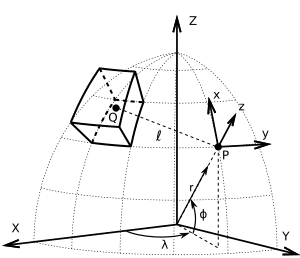
\includegraphics[width=0.6\linewidth]{figures/tesseroid-uieda.pdf}
\caption{
    A tesseroid (spherical prism) in a geocentric spherical coordinate system, with a
    computation point $P$ and its local north oriented Cartesian coordinate system.
    After \citet{Uieda2015}.
}
\label{fig:tesseroid}
\end{figure}

The main challenge of the GLQ integration is \DIFaddbegin \DIFadd{the }\DIFaddend loss of accuracy \DIFaddbegin \DIFadd{that occurs }\DIFaddend when the
computation point \DIFdelbegin \DIFdel{gets closer to }\DIFdelend \DIFaddbegin \DIFadd{approaches }\DIFaddend the tesseroid \citep{Ku1977}.
\citet{Uieda2016} built on the \DIFaddbegin \DIFadd{three dimensional }\DIFaddend adaptive discretization algorithm of
\citet{Li2011} to automatically obtain integration results with 0.1\% accuracy.
The algorithm \DIFdelbegin \DIFdel{consist in recursively splitting }\DIFdelend \DIFaddbegin \DIFadd{recursively divides }\DIFaddend the tesseroid into smaller ones when a
threshold is exceeded,
namely when the normalized distance to the computation point is greater than a
``distance-size ratio'' \DIFaddbegin \DIFadd{parameter }\DIFaddend ($D$).
\citet{Uieda2016} have also obtained standard values of $D$
for the gravitational potential, \DIFdelbegin \DIFdel{acceleration, and gradient }\DIFdelend \DIFaddbegin \DIFadd{its gradient and Marussi }\DIFaddend tensor components
by comparing the numerical \DIFdelbegin \DIFdel{model }\DIFdelend \DIFaddbegin \DIFadd{integration results }\DIFaddend with the fields generated by a spherical
shell.

\DIFaddbegin \DIFadd{Two recent publications present alternative approaches for calculating the gravitational
fields of homogeneous tesseroids and incorporate methodologies for tesseroids with
variable densities in depth.
\mbox{%DIFAUXCMD
\citet{Fukushima2018} }\hspace{0pt}%DIFAUXCMD
analytically integrates the volumetric integral for the
gravitational potential in the radial direction, obtaining a surface integral, which is
then numerically solved by conditionally splitting the tesseroid and applying the double
exponential quadrature rule.
The gradient of the potential and the Marussi tensor components are computed by finite
differences.
\mbox{%DIFAUXCMD
\citet{Fukushima2018} }\hspace{0pt}%DIFAUXCMD
also generalized their method to tesseroids with a radial
polynomial density function of arbitrary degree.
\mbox{%DIFAUXCMD
\citet{Lin2018} }\hspace{0pt}%DIFAUXCMD
compared the different integration and discretization methodologies for
homogeneous tesseroids.
From this analysis they developed a combined method:
for computation points near the tesseroid, they use a GLQ integration with an adaptive
discretization based on \mbox{%DIFAUXCMD
\citet{Uieda2016} }\hspace{0pt}%DIFAUXCMD
but only applied to the horizontal dimensions.
If the computation point is farther than a certain truncation distance,
a second order Taylor series approximation is applied instead along with the regular
subdivision developed by \mbox{%DIFAUXCMD
\citet{Grombein2013}}\hspace{0pt}%DIFAUXCMD
.
\mbox{%DIFAUXCMD
\citet{Lin2018} }\hspace{0pt}%DIFAUXCMD
also introduced a variation of their combined method to compute the
gravitational fields generated by tesseroids with a linearly varying density in the
radial dimension.
}

\DIFadd{Both the \mbox{%DIFAUXCMD
\citet{Lin2018} }\hspace{0pt}%DIFAUXCMD
and the \mbox{%DIFAUXCMD
\citet{Fukushima2018} }\hspace{0pt}%DIFAUXCMD
studies limit the radial density
variation to polynomial functions.
While most continuous and smooth functions can be approximated by piecewise linear
functions, the choice of a discretization interval is neither straight forward nor
automatic.
Furthermore, it is well known that the use of high-degree polynomials to approximate a
highly variable function produces unstable results when extrapolating beyond the data
domain.
These shortcomings could make piecewise linear or high-degree polynomial density
functions unwieldy for non-linear gravity inversions \mbox{%DIFAUXCMD
\citep[e.g.][]{Uieda2017} }\hspace{0pt}%DIFAUXCMD
if the
density function in depth is highly variable.
}

\DIFaddend We present a new algorithm for computing the gravitational \DIFdelbegin \DIFdel{fields generated by any
}\DIFdelend \DIFaddbegin \DIFadd{potential and its gradient
generated by a }\DIFaddend tesseroid with an arbitrary continuous density function on \DIFdelbegin \DIFdel{any }\DIFdelend \DIFaddbegin \DIFadd{an }\DIFaddend external
point.
It is based on the \DIFdelbegin \DIFdel{GLQ approximation and }\DIFdelend \DIFaddbegin \DIFadd{three dimensional GLQ integration, a two dimensional version of }\DIFaddend the
adaptive discretization of \citet{Uieda2016} \DIFdelbegin \DIFdel{, which we extend to include }\DIFdelend \DIFaddbegin \DIFadd{(following \mbox{%DIFAUXCMD
\citet{Lin2018}}\hspace{0pt}%DIFAUXCMD
),
and }\DIFaddend a new density-based \DIFdelbegin \DIFdel{discretization step.
In order to }\DIFdelend \DIFaddbegin \DIFadd{radial discretization algorithm.
To }\DIFaddend ensure the accuracy of the numerical approximation\DIFdelbegin \DIFdel{we have
determined }\DIFdelend \DIFaddbegin \DIFadd{, we empirically determine
}\DIFaddend optimal values for the controlling parameters by comparing the numerical \DIFdelbegin \DIFdel{approximation }\DIFdelend \DIFaddbegin \DIFadd{results }\DIFaddend with
analytical solutions for spherical shells.
Finally, we \DIFdelbegin \DIFdel{applied }\DIFdelend \DIFaddbegin \DIFadd{apply }\DIFaddend the methodology to model the Neuqu\'en basin, Argentina, using
tesseroids with \DIFdelbegin \DIFdel{an }\DIFdelend \DIFaddbegin \DIFadd{linear and }\DIFaddend exponentially increasing density with depth.


%%%%%%%%%%%%%%%%%%%%%%%%%%%%%%%%%%%%%%%%%%%%%%%%%%%%%%%%%%%%%%%%%%%%%%%%%%%%%%

\section{Methodology}

\DIFaddbegin \DIFadd{Consider a tesseroid in a geocentric spherical coordinate system defined by
pairs of geocentric latitudinal ($\phi_1$, $\phi_2$), longitudinal ($\lambda_1$,
$\lambda_2$), and radial ($r_1$, $r_2$) boundaries.
}\DIFaddend We define an external computation point $P(r, \phi, \lambda)$ \DIFdelbegin \DIFdel{in a geocentric spherical
coordinate system at a }\DIFdelend \DIFaddbegin \DIFadd{located at }\DIFaddend radius $r$,
geocentric latitude $\phi$, and longitude $\lambda$\DIFdelbegin \DIFdel{where the gravitational fields are going to be calculated.
The first and second }\DIFdelend \DIFaddbegin \DIFadd{.
\mbox{%DIFAUXCMD
\citet{Grombein2013} }\hspace{0pt}%DIFAUXCMD
provide efficient formulations for the volume integrals of the
gravitational potential and its first- and second-order derivatives of a tesseroid with
homogeneous density.
The }\DIFaddend derivatives of the gravitational potential are taken with
respect to the local north-oriented Cartesian coordinate system \DIFdelbegin \DIFdel{of }\DIFdelend \DIFaddbegin \DIFadd{with origin at }\DIFaddend $P$
(Fig.~\ref{fig:tesseroid}).
\DIFdelbegin \DIFdel{\mbox{%DIFAUXCMD
\citet{Grombein2013} }\hspace{0pt}%DIFAUXCMD
provide efficient formulations for the volume integrals of the
gravitational potential and its first and second derivatives of a tesseroid with
homogeneous density.
}\DIFdelend Here, we will assume that the tesseroid has a density varying with $r$ according to an
arbitrary \DIFaddbegin \DIFadd{continuous }\DIFaddend function $\rho(r)$.
Thus, the integrals for the gravitational \DIFdelbegin \DIFdel{fields }\DIFdelend \DIFaddbegin \DIFadd{potential and its first-order derivatives }\DIFaddend are
slightly modified to

\begin{equation}
    V(r,\phi,\lambda) = G
    \int\limits_{\lambda_1}^{\lambda_2}
    \int\limits_{\phi_1}^{\phi_2}
    \int\limits_{r_1}^{r_2}
    \frac{\rho(r')}{\ell} \kappa \,  dr' d\phi' d\lambda',
\label{eq:tesseroid-pot}
\end{equation}

\DIFdelbegin \begin{displaymath}
    \DIFdel{g_{\alpha}(r,\phi,\lambda) = G
    \int\limits_{\lambda_1}^{\lambda_2}
    \int\limits_{\phi_1}^{\phi_2}
    \int\limits_{r_1}^{r_2}
    \rho(r') \frac{\Delta_\alpha}{\ell^3}
    \kappa \, dr' d\phi' d\lambda',
%DIFDELCMD < \label{eq:tesseroid-grav}%%%
}\end{displaymath}%DIFAUXCMD
%DIFDELCMD < 

%DIFDELCMD < %%%
\DIFdelend \noindent and

\begin{equation}
    g\DIFdelbegin \DIFdel{_{\alpha\beta}}\DIFdelend \DIFaddbegin \DIFadd{_{\alpha}}\DIFaddend (r,\phi,\lambda) = G
    \int\limits_{\lambda_1}^{\lambda_2}
    \int\limits_{\phi_1}^{\phi_2}
    \int\limits_{r_1}^{r_2}
    \rho(r') \DIFdelbegin \DIFdel{I_{\alpha\beta} \, }\DIFdelend \DIFaddbegin \DIFadd{\frac{\Delta_\alpha}{\ell^3}
    }\DIFaddend \kappa \, dr' d\phi' d\lambda',
\DIFdelbegin %DIFDELCMD < \label{eq:tesseroid-tensor}
%DIFDELCMD < %%%
\DIFdelend \DIFaddbegin \label{eq:tesseroid-grav}
\DIFaddend \end{equation}

\noindent in which \DIFdelbegin %DIFDELCMD < 

%DIFDELCMD < %%%
\begin{displaymath}
    \DIFdel{I_{\alpha\beta} =
    \left(
        \frac{3\Delta_{\alpha} \Delta_{\beta}}{\ell^5} -
        \frac{\delta_{\alpha\beta}}{\ell^3}
    \right) ,
    %DIFDELCMD < \label{eq:tesseroid-tensor-kernel}%%%
}\end{displaymath}%DIFAUXCMD
%DIFDELCMD < 

%DIFDELCMD < \noindent %%%
\DIFdel{$\alpha, \beta \in \{x, y, z\}$,
$\delta_{\alpha\beta}$ is Kronecker's delta,
}\DIFdelend \DIFaddbegin \DIFadd{$\alpha \in \{x, y, z\}$,
}\DIFaddend $G = 6.674\times10^{-11}\, \text{m$^3$kg$^{-1}$s$^{-1}$}$ is the gravitational constant
and

\begin{equation}
    \Delta_x = r'[\cos\phi\sin\phi' - \sin\phi\cos\phi'
               \cos(\lambda' - \lambda)],
\end{equation}
\begin{equation}
    \Delta_y = r' \cos \phi' \sin(\lambda' - \lambda),
\end{equation}
\begin{equation}
    \Delta_z = r' \cos \psi - r,
\end{equation}
\begin{equation}
    \kappa = {r'}^2 \cos \phi',
\end{equation}
\begin{equation}
    \ell = \sqrt{{r'}^2 + r^2 - 2 r r' \cos \psi},
\label{eq:ell}
\end{equation}
\begin{equation}
    \cos\psi = \sin\phi\sin\phi' + \cos\phi\cos\phi'
                 \cos(\lambda' - \lambda).
\label{eq:cospsi}
\end{equation}


\subsection{Gauss-Legendre Quadrature integration}

Applying a $N$th order GLQ, we can approximate each integral in
equations\DIFdelbegin \DIFdel{\ref{eq:tesseroid-pot}, \ref{eq:tesseroid-grav} and\ref{eq:tesseroid-tensor} }\DIFdelend \DIFaddbegin \DIFadd{~\ref{eq:tesseroid-pot} and~\ref{eq:tesseroid-grav} }\DIFaddend by a weighted sum of the
integration kernel evaluated on the roots of an $N$th order Legendre polynomial
\citep[p.~390]{Hildebrand1987}.
Unlike the homogeneous density case, the radial density function $\rho(r)$ must also be
included in the integration and evaluated on the Legendre polynomial roots
(i.e.\DIFdelbegin \DIFdel{,
}\DIFdelend \DIFaddbegin \DIFadd{~}\DIFaddend quadrature nodes).

\DIFdelbegin %DIFDELCMD < \iftwocol{
%DIFDELCMD < \begin{displaymath}
%DIFDELCMD <     \begin{split}
%DIFDELCMD <         \iiint\limits_\Omega \rho(r') f(r', \phi', \lambda')
%DIFDELCMD <         d\Omega \approx& \\
%DIFDELCMD <         A
%DIFDELCMD <         \sum\limits_{i=1}^{N^r}
%DIFDELCMD <         \sum\limits_{j=1}^{N^\phi}
%DIFDELCMD <         \sum\limits_{k=1}^{N^\lambda}
%DIFDELCMD <         & W_i^r W_j^\phi W_k^\lambda \rho(r_i) f(r_i, \phi_j, \lambda_k),
%DIFDELCMD <     \end{split}
%DIFDELCMD < \label{eq:glq-var-dens}
%DIFDELCMD < \end{displaymath}
%DIFDELCMD < }{
%DIFDELCMD < \begin{displaymath}
%DIFDELCMD <     \iiint\limits_\Omega \rho(r') f(r', \phi', \lambda') d\Omega \approx
%DIFDELCMD <     A
%DIFDELCMD <     \sum\limits_{i=1}^{N^r}
%DIFDELCMD <     \sum\limits_{j=1}^{N^\phi}
%DIFDELCMD <     \sum\limits_{k=1}^{N^\lambda}
%DIFDELCMD <     W_i^r W_j^\phi W_k^\lambda \rho(r_i) f(r_i, \phi_j, \lambda_k),
%DIFDELCMD < \label{eq:glq-var-dens}
%DIFDELCMD < \end{displaymath}
%DIFDELCMD < }
%DIFDELCMD < %%%
\DIFdelend \DIFaddbegin \iftwocol{
\begin{equation}
    \begin{split}
        \int\limits_{\lambda_1}^{\lambda_2}
        \int\limits_{\phi_1}^{\phi_2}
        \int\limits_{r_1}^{r_2}
        \rho(r') f(r', \phi', \lambda')
        dr' d\phi' d\lambda' \approx& \\
        A
        \sum\limits_{i=1}^{N^r}
        \sum\limits_{j=1}^{N^\phi}
        \sum\limits_{k=1}^{N^\lambda}
        W_i^r W_j^\phi W_k^\lambda
        &\rho(r_i) f(r_i, \phi_j, \lambda_k),
    \end{split}
\label{eq:glq-var-dens}
\end{equation}
}{
\begin{equation}
    \int\limits_{\lambda_1}^{\lambda_2}
    \int\limits_{\phi_1}^{\phi_2}
    \int\limits_{r_1}^{r_2}
    \rho(r') f(r', \phi', \lambda')
    dr' d\phi' d\lambda' \approx
    A
    \sum\limits_{i=1}^{N^r}
    \sum\limits_{j=1}^{N^\phi}
    \sum\limits_{k=1}^{N^\lambda}
    W_i^r W_j^\phi W_k^\lambda \rho(r_i) f(r_i, \phi_j, \lambda_k),
\label{eq:glq-var-dens}
\end{equation}
}
\DIFaddend 

\noindent where

\begin{equation}
    A = \frac{(\lambda_2 - \lambda_1)(\phi_2 - \phi_1)(r_2 - r_1)}{8},
\end{equation}

\noindent \DIFaddbegin \DIFadd{$f(r', \phi', \lambda')$ is an integral kernel for a homogeneous tesseroid
\mbox{%DIFAUXCMD
\citep{Grombein2013}}\hspace{0pt}%DIFAUXCMD
,
}\DIFaddend $(r_i, \phi_j, \lambda_k)$ are the \DIFaddbegin \DIFadd{coordinates of the }\DIFaddend quadrature nodes,
\DIFaddbegin \DIFadd{$N^r$, $N^\phi$, $M^\lambda$ are the quadrature orders }\DIFaddend and $W_i^r$\DIFaddbegin \DIFadd{, $W_j^\phi$,
$W_k^\lambda$ }\DIFaddend are the quadrature weights \DIFdelbegin \DIFdel{.
}\DIFdelend \DIFaddbegin \DIFadd{in the radial, latitudinal, and longitudinal
directions, respectively.
\mbox{%DIFAUXCMD
\citet[p.~391]{Hildebrand1987} }\hspace{0pt}%DIFAUXCMD
provides the formulas for calculating the GLQ weights and
pre-computed values of the Legendre polynomial roots for low orders.
See \mbox{%DIFAUXCMD
\citet{Uieda2016} }\hspace{0pt}%DIFAUXCMD
for a more detailed description using a similar notation to the
one used here.
It is worth noting that a GLQ is equivalent to approximating the tesseroid by $N^r
\times N^\phi \times N^\lambda$ point masses located on the quadrature nodes
\mbox{%DIFAUXCMD
\citep{Ku1977, Asgharzadeh2007}}\hspace{0pt}%DIFAUXCMD
.
}\DIFaddend 


\subsection{\DIFaddbegin \DIFadd{Two Dimensional }\DIFaddend Adaptive Discretization}

\citet{Ku1977} noticed that the GLQ integration
becomes less accurate when the computation point is closer to the
mass element.
One way to prevent this from happening would be to increase the GLQ order.
Doing so would uniformly increase the number of point masses inside the
tesseroid volume.
However, an increase in the point mass concentration is only required close to the
computation point \citep{Uieda2016}.
Alternatively, \citet{Li2011} proposed an adaptive
discretization algorithm which keeps the GLQ order fixed and divides the
tesseroid based on a ratio between the distance to the computation
point and its dimensions.
This algorithm produces a more efficient computation because an increased concentration
of point masses is produced where it is needed more.
\citet{Uieda2016} developed a modified version of this algorithm \DIFdelbegin \DIFdel{, which we will use
here}\DIFdelend \DIFaddbegin \DIFadd{along with an efficient
computational implementation.
Both algorithms perform tesseroid subdivisions in the latitudinal,
longitudinal and radial directions, thus we can define them as three-dimensional
adaptive discretization algorithms.
On the other hand, \mbox{%DIFAUXCMD
\citet{Lin2018} }\hspace{0pt}%DIFAUXCMD
proposed a two dimensional discretization algorithm
that subdivides the tesseroid only on the latitudinal and longitudinal directions.
Removing a dimension from the discretization makes the computation more efficient by
reducing the number of tesseroids in the model, while
retaining an acceptable accuracy \mbox{%DIFAUXCMD
\citep{Lin2018}}\hspace{0pt}%DIFAUXCMD
.
}

\DIFadd{Here we will follow \mbox{%DIFAUXCMD
\citet{Lin2018} }\hspace{0pt}%DIFAUXCMD
and use a two dimensional version of the adaptive
discretization of \mbox{%DIFAUXCMD
\citet{Uieda2016}}\hspace{0pt}%DIFAUXCMD
}\DIFaddend .
What follows is a summary of the algorithm and the reader is referred to
\citet{Uieda2016} for a detailed description.

\DIFdelbegin \DIFdel{The following algorithm computes the gravitational fields at a given point at $(r, \phi,
\lambda)$ due to a tesseroid with its geometric centre at $(r_t, \phi_t, \lambda_t)$ and
dimensions $L_r$, $L_\phi$, and $L_\lambda$ given by
}%DIFDELCMD < 

%DIFDELCMD < %%%
\begin{displaymath}
    \DIFdel{L_\lambda = r_2 \arccos(\sin^2\phi_t +
        \cos^2\phi_t\cos(\lambda_2 - \lambda_1)),
    %DIFDELCMD < \label{eq:sizelon}%%%
}\end{displaymath}%DIFAUXCMD
%DIFDELCMD < 

%DIFDELCMD < %%%
\begin{displaymath}
    \DIFdel{L_\phi = r_2 \arccos(\sin\phi_2\sin\phi_1 + \cos\phi_2\cos\phi_1),
}\end{displaymath}%DIFAUXCMD
%DIFDELCMD < 

%DIFDELCMD < %%%
\DIFdel{and
}%DIFDELCMD < 

%DIFDELCMD < %%%
\begin{displaymath}
    \DIFdel{L_r = r_2 - r_1.
    %DIFDELCMD < \label{eq:sizer}%%%
}\end{displaymath}%DIFAUXCMD
%DIFDELCMD < 

%DIFDELCMD < %%%
\DIFdelend \textit{Step 1}: Check that the tesseroid satisfies the following inequality for each
dimension \DIFdelbegin \DIFdel{$L_i$ }\DIFdelend \DIFaddbegin \DIFadd{$L_i\ (i \in \{\lambda, \phi\})$ }\DIFaddend of the tesseroid:

\begin{equation}
    \frac{d}{L_i} \geq D,
    \label{eq:condition}
\end{equation}

\noindent
in which $D$ is a positive scalar called the distance-size ratio\DIFdelbegin \DIFdel{and }\DIFdelend \DIFaddbegin \DIFadd{, }\DIFaddend $d$ is the distance
between the computation point and the geometric centre of the tesseroid

\begin{equation}
    d = \left[
        r^2 + r_t^2 - 2 r r_t \cos\psi_t
        \right]^{\frac{1}{2}} ,
    \label{eq:distance}
\end{equation}

\begin{equation}
    \cos\psi_t =
        \sin\phi\sin\phi_t + \cos\phi\cos\phi_t\cos(\lambda - \lambda_t).
\end{equation}

\DIFaddbegin \begin{equation}
    \DIFadd{r_t = \frac{r_2 + r_1}{2}, \quad
    \phi_t = \frac{\phi_2 + \phi_1}{2}, \quad
    \lambda_t = \frac{\lambda_2 + \lambda_1}{2}.
}\end{equation}

\noindent
\DIFadd{and the dimensions of the tesseroid are defined as
}

\begin{equation}
    \DIFadd{L_\lambda = r_2 \arccos(\sin^2\phi_t +
        \cos^2\phi_t\cos(\lambda_2 - \lambda_1)),
    \label{eq:sizelon}
}\end{equation}

\noindent \DIFadd{and
}

\begin{equation}
    \DIFadd{L_\phi = r_2 \arccos(\sin\phi_2\sin\phi_1 + \cos\phi_2\cos\phi_1).
}\end{equation}

\DIFaddend \textit{Step 2}:
If none of the dimensions of the tesseroid fail inequality\DIFaddbegin \DIFadd{~}\DIFaddend \ref{eq:condition}, then
compute the gravitational effect of the tesseroid using a second-order GLQ
(Eq.\DIFaddbegin \DIFadd{~}\DIFaddend \ref{eq:glq-var-dens}).
Add the computed effect to a running total.

\textit{Step 3}:
If \DIFdelbegin \DIFdel{any dimension fails inequality\ref{eq:condition}}\DIFdelend \DIFaddbegin \DIFadd{inequality~\ref{eq:condition} does not hold for one of the dimensions
(longitudinal or latitudinal)}\DIFaddend , split the tesseroid in half along \DIFdelbegin \DIFdel{the offending dimensions}\DIFdelend \DIFaddbegin \DIFadd{that dimension}\DIFaddend .
Repeat steps 1-3 for all smaller tesseroids until none are left \DIFaddbegin \DIFadd{that violate
inequality~\ref{eq:condition}}\DIFaddend .

\textit{Final step}:
By the end of the algorithm, \DIFaddbegin \DIFadd{a second-order GLQ will have been applied to each smaller
tesseroid and }\DIFaddend the running total \DIFaddbegin \DIFadd{gathered in step 2 }\DIFaddend will be the gravitational effect of
the \DIFaddbegin \DIFadd{original }\DIFaddend tesseroid.

\DIFdelbegin \DIFdel{Notice that the }\DIFdelend \DIFaddbegin \DIFadd{The }\DIFaddend distance-size ratio $D$ determines how many times the tesseroids will be divided.
Therefore, it effectively regulates both the accuracy of the algorithm and its
computation time.
An optimal value for $D$ cannot be directly calculated from the desired accuracy level.
Instead, it is empirically determined by comparing the numerical results with the
analytical solution for a spherical shell.
\citet{Uieda2016} used a shell with homogeneous density to determine optimal values of
$D$.
Here, we will repeat the numerical experiment using analytical expressions for shells
with density varying according to \DIFdelbegin \DIFdel{exponential and linear }\DIFdelend functions of $r$.
\DIFaddbegin \DIFadd{This experiment will also test whether the same values of $D$ determined by
\mbox{%DIFAUXCMD
\citet{Uieda2016} }\hspace{0pt}%DIFAUXCMD
can be used for the two dimensional adaptive discretization.
}\DIFaddend 


\subsection{Density-based Discretization Algorithm}

\begin{figure*}
\centering
\includegraphics[width=\linewidth]
    {figures/density-based-discretization-algorithm.pdf}
\caption{
    Example application of the density-based discretization algorithm to a non-linear
    density function.
    (a)\DIFdelbeginFL \DIFdelFL{the }\DIFdelendFL \DIFaddbeginFL \DIFaddFL{~The }\DIFaddendFL normalised density function $\rho_n(r')$ (blue), current boundaries of the
    tesseroid (orange dots), and the linear density function $\rho_l(r')$ (orange line).
    The dashed red line represents the maximum density difference $\Delta \rho (r')$ at
    which the tesseroid would be divided (assuming that the
    inequality\DIFaddbeginFL \DIFaddFL{~}\DIFaddendFL \ref{eq:delta-density} is not satisfied).
    (b)\DIFdelbeginFL \DIFdelFL{second }\DIFdelendFL \DIFaddbeginFL \DIFaddFL{~Second }\DIFaddendFL iteration of the algorithm with a new linear density function and maximum
    density difference. The tesseroid would be divided at the depth indicated by the
    dashed red line.
    (c)\DIFdelbeginFL \DIFdelFL{third }\DIFdelendFL \DIFaddbeginFL \DIFaddFL{~Third }\DIFaddendFL iteration of the algorithm.
    (d)\DIFdelbeginFL \DIFdelFL{final }\DIFdelendFL \DIFaddbeginFL \DIFaddFL{~Final }\DIFaddendFL output of the density-based discretization, assuming that all four new
    tesseroids satisfy inequality\DIFaddbeginFL \DIFaddFL{~}\DIFaddendFL \ref{eq:delta-density}.
}
\label{fig:density-discretization-algorithm}
\end{figure*}

The numerical integration of an arbitrary \DIFaddbegin \DIFadd{continuous }\DIFaddend density function introduces a new
type of problem: the integration error from using only a few \DIFdelbegin \DIFdel{nodes to discretize the }\DIFdelend \DIFaddbegin \DIFadd{quadrature nodes to account
for the variation of the }\DIFaddend density function.
The \DIFaddbegin \DIFadd{three dimensional }\DIFaddend adaptive discretization may help to reduce this kind of error \DIFaddbegin \DIFadd{by
adding more point masses in the radial direction}\DIFaddend .
However, it does not take into account the density function \DIFaddbegin \DIFadd{itself when dividing the
tesseroid }\DIFaddend and hence it is not well suited to fully perform this task.

We have developed a complementary discretization algorithm \DIFaddbegin \DIFadd{in the redial direction }\DIFaddend that
takes into account the variations of the density function.
This density-based discretization \DIFdelbegin \DIFdel{happens }\DIFdelend \DIFaddbegin \DIFadd{is applied }\DIFaddend prior to the \DIFaddbegin \DIFadd{two dimensional }\DIFaddend adaptive
discretization described in the previous section.
In short, the algorithm divides the tesseroid along the radial dimension at the
depths at which the \emph{maximum density variations} take place.

Consider an \emph{original} tesseroid with \DIFaddbegin \DIFadd{a }\DIFaddend density given by the \DIFaddbegin \DIFadd{continuous }\DIFaddend function
$\rho(r')$.
Before the density-based discretization starts,
we normalise the density function to the range $[0, 1]$ as follows

\begin{equation}
    \rho_n(r') =
    \frac{\rho(r') - \rho_\text{min}}{\rho_\text{max} - \rho_\text{min}},
\end{equation}

\noindent in which $\rho_\text{min}$ and $\rho_\text{max}$ are the minimum and maximum
density values inside the tesseroid boundaries.
We emphasize that this normalised density function will not be modified throughout the
algorithm.
In case the density function is constant, both maximum and minimum densities will be
equal and the density-based discretization algorithm will not be applied.

The algorithm is comprised of the following steps
(Fig.\DIFaddbegin \DIFadd{~}\DIFaddend \ref{fig:density-discretization-algorithm}):

\textit{Step 1}:
Define a linear function $\rho_l(r')$ that assumes the same values as the normalised
density \DIFaddbegin \DIFadd{function }\DIFaddend $\rho_n(r')$ at the boundaries of the tesseroid ($r_1$ and $r_2$):

\begin{equation}
    \rho_l(r') =
    \frac{ \rho_n(r_2) - \rho_n(r_1) }{ r_2 - r_1 } (r' - r_1) + \rho_n(r_1),
    \label{eq:density-reference-line}
\end{equation}

\textit{Step 2}:
Evaluate the normalized and linear density functions on a range of $N$ radii between
$r_1$ and $r_2$.
We have opted for $N = 101$ but the specific value of $N$ is not critical to the
algorithm.

\textit{Step 3}:
Compute the absolute difference between the values of the linear and normalised density
functions:

\begin{equation}
    \Delta \rho (r') = | \rho_n(r') - \rho_l(r') |.
    \label{eq:density-abs-diff}
\end{equation}

\textit{Step 4}:
If the following inequality holds, the tesseroid will not be divided:

\begin{equation}
    \text{max}\{ \Delta \rho(r') \} \frac{L_r}{L_r^\text{orig}} \le \delta,
    \label{eq:delta-density}
\end{equation}

\noindent
in which $L_r$ is the radial dimension of the tesseroid being considered for division,
\DIFaddbegin 

\begin{equation}
    \DIFadd{L_r = r_2 - r_1,
}\end{equation}

\noindent \DIFaddend $L_r^\text{orig}$ is the radial dimension of the original tesseroid, and
$\delta$ is a positive constant henceforth called the \textit{delta ratio}.

\textit{Step 5}:
If inequality\DIFaddbegin \DIFadd{~}\DIFaddend \ref{eq:delta-density} is not satisfied, then the tesseroid is split in
two parts at the radius $r_\text{max}$ at which the maximum absolute difference
(Eq.\DIFaddbegin \DIFadd{~}\DIFaddend \ref{eq:density-abs-diff}) takes place.
\DIFdelbegin %DIFDELCMD < 

%DIFDELCMD < %%%
\textit{\DIFdel{Step 6}}%DIFAUXCMD
\DIFdel{:
Repeat steps 1-6 }\DIFdelend \DIFaddbegin \DIFadd{Repeat steps 1-5 }\DIFaddend for each smaller tesseroid produced in \DIFdelbegin \DIFdel{step 5.
}\DIFdelend \DIFaddbegin \DIFadd{this step.
}\DIFaddend 

\DIFaddbegin \textit{\DIFadd{Final step}}\DIFadd{:
}\DIFaddend Once all smaller tesseroids satisfy \DIFdelbegin \DIFdel{Eq.}\DIFdelend \DIFaddbegin \DIFadd{inequality.~}\DIFaddend \ref{eq:delta-density}, each one is
subjected to the \DIFaddbegin \DIFadd{two dimensional }\DIFaddend adaptive discretization algorithm described earlier to
calculate their gravitational effects.

On the first iteration, the ratio $L_r/L_r^\text{orig} = 1$ because the tesseroid being
divided is the original one.
For \DIFdelbegin \DIFdel{future }\DIFdelend \DIFaddbegin \DIFadd{further }\DIFaddend iterations, the ratio will be progressively smaller than one as the
tesseroids get smaller.
This is intended to limit the number of divisions to the ones that will
significantly reduce the numerical error:
dividing a large tesseroid with a small $\text{max}\{ \Delta \rho(r') \}$ would
improve the integration accuracy more than dividing a small tesseroid with a
higher $\text{max}\{ \Delta \rho(r') \}$.
\DIFdelbegin \DIFdel{We also do not divide tesseroids with $L_r < 1$ mm because any integration errors would
be negligible due to the small mass of the tesseroid..
}\DIFdelend 

The higher $\delta$ is, the fewer divisions will be made, and vice-versa.
Thus, it controls how many times the tesseroids will be divided based on the density
function and, indirectly, determines the accuracy and computation time of
numerical integration.
This raises the need to determine a maximum value of $\delta$ that
ensures an acceptable accuracy while minimising the computation time.


\DIFaddbegin \subsection{\DIFadd{Algorithm summary}}

\DIFadd{In summary, given a tesseroid with density varying in depth according to an arbitrary
continuous function, we propose the following steps to numerically compute its
gravitational fields on an external point:
}

\textit{\DIFadd{Step 1:}}
\DIFadd{Apply the density-based discretization algorithm to discretize the tesseroid in the
radial dimension, producing a set of tesseroids with the same longitudinal and
latitudinal dimensions as the original one but with different radial boundaries.
}

\textit{\DIFadd{Step 2:}}
\DIFadd{Apply the two dimensional adaptive discretization algorithm for each tesseroid obtained
in the previous step.
If needed, the algorithm will divide each tesseroid in the latitudinal and longitudinal
direction, generating a set of smaller tesseroids.
}

\textit{\DIFadd{Step 3:}}
\DIFadd{Apply a second-order GLQ to numerically compute the gravitational fields
(Eq.~\ref{eq:glq-var-dens}) generated by each tesseroid obtained in the
previous step.
The numerical integration includes the density function and can be applied
without modification to any continuous function.
The sum of these results is the gravitational field of the original tesseroid.
}


\DIFaddend \subsection{Software implementation}

We have implemented the algorithms described in the previous sections in the Python
programming language.
The software is based on the \DIFdelbegin \DIFdel{pre-existing code for the homogeneous density tesseroid
\mbox{%DIFAUXCMD
\citep{Uieda2016}}\hspace{0pt}%DIFAUXCMD
, more specifically the implementation in the Python library }\DIFdelend \DIFaddbegin \DIFadd{Python implementation of \mbox{%DIFAUXCMD
\citet{Uieda2016} }\hspace{0pt}%DIFAUXCMD
that is included
in the }\DIFaddend Fatiando a Terra \DIFaddbegin \DIFadd{library }\DIFaddend v0.5 \citep{Uieda2013}.
The more time consuming parts of the algorithm are written in the Cython language to
achieve higher performance.
\DIFaddbegin \DIFadd{We leverage the dynamic nature of the Python language to allow user-defined radial
density functions as inputs to the software.
Thus, our code can evaluate linear, exponential, polynomial, sinusoidal, cubic splines,
or any other continuous density function without modification.
}\DIFaddend This new code is freely available under the BSD 3-clause open-source license.
It can be \DIFaddbegin \DIFadd{freely }\DIFaddend downloaded from the online repository
\href{https://github.com/pinga-lab/tesseroid-variable-density}{github.com/pinga-lab/tesseroid-variable-density}.



%%%%%%%%%%%%%%%%%%%%%%%%%%%%%%%%%%%%%%%%%%%%%%%%%%%%%%%%%%%%%%%%%%%%%%%%%%%%%

\section{Determination of the distance-size and delta ratios}

The distance-size ratio $D$ of the adaptive discretization and the delta ratio $\delta$
of the density-based discretization determine how many times each tesseroid will be
divided and thus indirectly control the numerical error of the integration.
Optimal values for $D$ and $\delta$ must be determined in order to ensure both
acceptable numerical accuracy and computation efficiency for the algorithm.

\citet{Uieda2016} compared the numerical integration of homogeneous density tesseroids
with the analytical solution of a spherical shell \DIFdelbegin \DIFdel{\mbox{%DIFAUXCMD
\citep{Mikuska2006,Grombein2013} }\hspace{0pt}%DIFAUXCMD
}\DIFdelend \DIFaddbegin \DIFadd{\mbox{%DIFAUXCMD
\citep{Mikuska2006, Grombein2013} }\hspace{0pt}%DIFAUXCMD
}\DIFaddend in
order to obtain default values for the distance-size ratio $D$.
We will follow this idea but for our needs the spherical shell must
have the same density function of radius as our tesseroid model.
\DIFdelbegin \DIFdel{Analytical solutions for a variable density spherical shell are not present in the literature and so they must be obtained first}\DIFdelend \DIFaddbegin \DIFadd{\mbox{%DIFAUXCMD
\citet{Lin2018} }\hspace{0pt}%DIFAUXCMD
show the analytical solution of the gravitational potential generated by
a spherical shell with linear density in the radial coordinate}\DIFaddend .
We derive \DIFdelbegin \DIFdel{the expressions }\DIFdelend \DIFaddbegin \DIFadd{an expression }\DIFaddend for the gravitational \DIFdelbegin \DIFdel{fields of spherical shells with
linear
and exponentialdensity functions of radius in Appendix\ref{sec:shell}}\DIFdelend \DIFaddbegin \DIFadd{potential of a spherical shell with
an arbitrary density function in depth (Eq.~\ref{eq:shell-pot}),
from which we obtained
expressions for linear, exponential, and sinusoidal density functions
(see Appendix~\ref{sec:shell})}\DIFaddend .

\DIFaddbegin \DIFadd{In order to compare the numerical results with the analytical solution we must build
spherical shell models out of tesseroids.
We divide the spherical shell along the latitudinal and longitudinal directions to
obtain a shell model made out of $6 \times 12 = 72$ tesseroids of size
$30^\circ \times 30^\circ$.
In order to asses the density-based discretization in the radial dimension,
we use spherical shell models with different thicknesses (Table~\ref{tab:shell-models}).
The thickness values were chosen to represent a range of applications, from topographic
to lithospheric scale models.
Because the amount of tesseroid divisions in the adaptive discretization will be
proportional to the tesseroid size (Eq.~\ref{eq:condition}),
some of these configurations represent worse-case scenarios.
Most practical applications will use tesseroids smaller than
$30^\circ \times 30^\circ \times 1000\ \text{km}$.
}

\DIFadd{The differences between the analytical and numerical solutions could be calculated on a
single computation point due to the rotational symmetry of the spherical shell.
However, the numerical results depend on the relative location between the computation
point and the tesseroid \mbox{%DIFAUXCMD
\citep{Ku1977, Asgharzadeh2007, Uieda2016}}\hspace{0pt}%DIFAUXCMD
.
We account for this effect by calculating the differences on regular grids and keeping
only the maximum absolute difference.
All calculations are repeated for four different computation grids
(Table~\ref{tab:grids}):
a local grid at the pole, a local grid at the equator, a global grid at zero height
above the shell, and a global grid at a height of 260 km (representing the nominal
height of the GOCE satellite).
These grids span a broad scenario of use cases and ensure an acceptable accuracy on each
one of them.
}

\DIFaddend We perform comparisons between the analytical solutions for the spherical shell and the
numerical integration results for linear\DIFdelbegin \DIFdel{and exponential}\DIFdelend \DIFaddbegin \DIFadd{, exponential, and sinusoidal }\DIFaddend density
functions.
\DIFaddbegin \DIFadd{The comparisons are repeated for all combinations of tesseroid models in
Table~\ref{tab:shell-models} and computation grids in Table~\ref{tab:grids}.
}\DIFaddend From these results, we generalize \DIFdelbegin \DIFdel{default }\DIFdelend \DIFaddbegin \DIFadd{optimal }\DIFaddend values for $D$ and $\delta$ that ensure a
numerical error lower than 0.1\% of the spherical shell values \DIFaddbegin \DIFadd{for most use cases}\DIFaddend .

\begin{table}
\caption{
    Description of the \DIFdelbeginFL \DIFdelFL{computation grids }\DIFdelendFL \DIFaddbeginFL \DIFaddFL{tesseroid models }\DIFaddendFL used to \DIFaddbeginFL \DIFaddFL{build spherical shells and }\DIFaddendFL characterize
    the accuracy of the numerical integration.
    \DIFdelbeginFL \DIFdelFL{All grids consist }\DIFdelendFL \DIFaddbeginFL \DIFaddFL{The outer radius ($R_2$) }\DIFaddendFL of \DIFdelbeginFL \DIFdelFL{a set }\DIFdelendFL \DIFaddbeginFL \DIFaddFL{every shell model is equal to the mean Earth radius
    (6378.137 km), while the inner radius ($R_1$) is determined by its thickness.
    The horizontal dimensions }\DIFaddendFL of \DIFdelbeginFL \DIFdelFL{$10 \times 10$ points}\DIFdelendFL \DIFaddbeginFL \DIFaddFL{the tesseroids and the total number of
    tesseroids in the shell model are given in the latitudinal and longitudinal
    dimensions, respectively}\DIFaddendFL .
}
\DIFaddbeginFL \label{tab:shell-models}
\begin{tabular}{rccccc}
    \DIFaddFL{Thickness }& \DIFaddFL{Tesseroid size }& \DIFaddFL{Number of tesseroids }\\ \hline
    \DIFaddFL{0.1 km  }& \DIFaddFL{$30^\circ \times 30^\circ$ }& \DIFaddFL{$6 \times 12 = 72$ }\\
    \DIFaddFL{1 km    }& \DIFaddFL{$30^\circ \times 30^\circ$ }& \DIFaddFL{$6 \times 12 = 72$ }\\
    \DIFaddFL{10 km   }& \DIFaddFL{$30^\circ \times 30^\circ$ }& \DIFaddFL{$6 \times 12 = 72$ }\\
    \DIFaddFL{100 km  }& \DIFaddFL{$30^\circ \times 30^\circ$ }& \DIFaddFL{$6 \times 12 = 72$ }\\
    \DIFaddFL{1000 km }& \DIFaddFL{$30^\circ \times 30^\circ$ }& \DIFaddFL{$6 \times 12 = 72$ }\\
\end{tabular}
\end{table}

\begin{table}
\caption{
    \DIFaddFL{Description of the computation grids used to characterize the accuracy of the
    numerical integration.
    Grid height is defined above the mean Earth radius.
}}
\DIFaddendFL \label{tab:grids}
\begin{tabular}{lccc}
    Name & Grid \DIFdelbeginFL \DIFdelFL{size }\DIFdelendFL \DIFaddbeginFL \DIFaddFL{spacing }\DIFaddendFL & Grid region (degrees) & Grid height (km)
    \\ \hline
    Pole      & \DIFdelbeginFL \DIFdelFL{$1^\circ \times 1^\circ$ }\DIFdelendFL \DIFaddbeginFL \DIFaddFL{$0.1^\circ$ }\DIFaddendFL &   \DIFdelbeginFL \DIFdelFL{$0\text{E}/1\text{E}/89\text{N}/90\text{N}$ }\DIFdelendFL \DIFaddbeginFL \DIFaddFL{0E /   1E / 89N / 90N }\DIFaddendFL & \DIFdelbeginFL \DIFdelFL{2 }\DIFdelendFL \DIFaddbeginFL \DIFaddFL{0   }\DIFaddendFL \\
    Equator   & \DIFdelbeginFL \DIFdelFL{$1^\circ \times 1^\circ$ }\DIFdelendFL \DIFaddbeginFL \DIFaddFL{$0.1^\circ$ }\DIFaddendFL &   \DIFdelbeginFL \DIFdelFL{$0\text{E}/1\text{E}/0\text{N}/1\text{N}$ }\DIFdelendFL \DIFaddbeginFL \DIFaddFL{0E /   1E /  0N / 1N  }\DIFaddendFL & \DIFdelbeginFL \DIFdelFL{2 }\DIFdelendFL \DIFaddbeginFL \DIFaddFL{0   }\DIFaddendFL \\
    \DIFdelbeginFL \DIFdelFL{Satellite }\DIFdelendFL \DIFaddbeginFL \DIFaddFL{Global    }\DIFaddendFL & \DIFdelbeginFL \DIFdelFL{$1^\circ \times 1^\circ$ }\DIFdelendFL \DIFaddbeginFL \DIFaddFL{$ 10^\circ$ }\DIFaddendFL & \DIFdelbeginFL \DIFdelFL{$0\text{E}/1\text{E}/89\text{N}/90\text{N}$ }\DIFdelendFL \DIFaddbeginFL \DIFaddFL{180W / 180E / 90S / 90N }\DIFaddendFL & \DIFdelbeginFL \DIFdelFL{260 }\DIFdelendFL \DIFaddbeginFL \DIFaddFL{0   }\DIFaddendFL \\
    \DIFdelbeginFL \DIFdelFL{Big Grid }\DIFdelendFL \DIFaddbeginFL \DIFaddFL{Satellite }\DIFaddendFL & \DIFdelbeginFL \DIFdelFL{$30^\circ \times 30^\circ$ }\DIFdelendFL \DIFaddbeginFL \DIFaddFL{$ 10^\circ$ }\DIFaddendFL & \DIFdelbeginFL \DIFdelFL{$0\text{E}/30\text{E}/60\text{N}/90\text{N}$ }\DIFdelendFL \DIFaddbeginFL \DIFaddFL{180W / 180E / 90S / 90N }\DIFaddendFL & \DIFdelbeginFL \DIFdelFL{2 }\DIFdelendFL \DIFaddbeginFL \DIFaddFL{260 }\DIFaddendFL \\
\end{tabular}
\end{table}


\subsection{Linear Density}

A spherical shell with a linear density function given by

\begin{equation}
    \rho(r') = ar' + b,
    \label{eq:density-linear}
\end{equation}

\noindent
has an analytical \DIFdelbegin \DIFdel{solution given by Eq.\ref{eq:shell-pot-linear}.
}\DIFdelend \DIFaddbegin \DIFadd{solutions for the gravitational potential and its vertical derivative
given by Eqs.~\ref{eq:shell-pot-linear} and~\ref{eq:shell-gz}.
The values of the angular and linear coefficients ($a$ and $b$)
can be chosen so that the density assumes the values of $\rho_\text{in} = 3300$~kg/m$^3$
and $\rho_\text{out} = 2670$~kg/m$^3$ on the inner ($R_\text{in}$) and outer
($R_\text{out}$) radii of the shell, respectively,
}\DIFaddend 

\DIFaddbegin \begin{equation}
    \DIFadd{a = \frac{\rho_\text{out} - \rho_\text{in}}{R_\text{out} - R_\text{in}},
}\end{equation}

\begin{equation}
    \DIFadd{b = \rho_\text{out} -
    \frac{\rho_\text{out} - \rho_\text{in}}{R_\text{out} - R_\text{in}} R_\text{out}.
}\end{equation}


\begin{figure*}
\centering
\includegraphics[width=\linewidth]{figures/linear-density-diffs.pdf}
\caption{
    \DIFaddFL{Differences between the gravitational fields generated by each tesseroid shell model
    and the analytical solution as a function of the distance-size ratio $D$.
    Each model has a linear density function (Eq.~\ref{eq:density-linear}).
    The computations were performed on the four grids described in Table~\ref{tab:grids}
    and using the shell models detailed in Table~\ref{tab:shell-models}.
    Each line represents the maximum absolute difference between the numerical results
    and the analytical solution for a given shell model.
    Due to the linearity of the density function, the density-based discretization
    algorithm is not applied.
    Differences are reported as a percentage of the analytical solutions.
    The horizontal dashed black line represents a target difference of 0.1\%.
}}
\label{fig:D-linear}
\end{figure*}

\DIFaddend The absolute density difference defined on equation\DIFaddbegin \DIFadd{~}\DIFaddend \ref{eq:density-abs-diff} will
always be zero for the linear density case.
As a result, the inequality\DIFaddbegin \DIFadd{~}\DIFaddend \ref{eq:delta-density} will always be satisfied and no
divisions will ever be performed \DIFaddbegin \DIFadd{during the density-based discretization}\DIFaddend .
Therefore, the \DIFdelbegin \DIFdel{distance-size ratio $D$ of the }\DIFdelend \DIFaddbegin \DIFadd{two dimensional }\DIFaddend adaptive discretization algorithm is the
only mechanism that controls the accuracy of the numerical integration \DIFaddbegin \DIFadd{for the linear
density case}\DIFaddend .
For this reason, we will \DIFaddbegin \DIFadd{ignore the values of $\delta$ and }\DIFaddend only determine the minimum
value of $D$ needed in order to guarantee an acceptable accuracy\DIFdelbegin \DIFdel{while ignoring the value of $\delta$}\DIFdelend .

\DIFdelbegin \DIFdel{In order to compare the numerical results with the analytical solution we
must build a spherical shell made of tesseroids.
The outer radius of the shell is equal to the mean Earth radius and we repeat the
calculations for shell thicknesses of 1km and 35km.
We discretize the shell into a single layer of $30^\circ \times 30^\circ$ tesseroids and
compute their gravitational effects on $10 \times 10$ point grids with different
resolutions, heights, and locations on the sphere.
These grids are defined in Table \ref{tab:grids}.
The density of the shell and tesseroid model varies linearly with $r$
(Eq. \ref{eq:density-linear}) with angular coefficient
}%DIFDELCMD < 

%DIFDELCMD < %%%
\begin{displaymath}
    \DIFdel{a = -\frac{3300\text{kg/m$^3$} - 2670\text{kg/m$^3$}}{R - R_1},
}\end{displaymath}%DIFAUXCMD
%DIFDELCMD < 

%DIFDELCMD < \noindent %%%
\DIFdel{and linear coefficient
}%DIFDELCMD < 

%DIFDELCMD < %%%
\begin{displaymath}
    \DIFdel{c = \frac{3300\text{kg/m$^3$} -
        2670\text{kg/m$^3$}}{R - R_1} R +
        2670\text{kg/m$^3$},
}\end{displaymath}%DIFAUXCMD
%DIFDELCMD < 

%DIFDELCMD < \noindent
%DIFDELCMD < %%%
\DIFdel{in which $R$ = 6378.137 km is the mean Earth radius and $R_1$ is the inner radius of the
shell (determined by the thickness).
}%DIFDELCMD < 

%DIFDELCMD < \begin{figure*}
%DIFDELCMD < \centering
%DIFDELCMD < \includegraphics[width=\linewidth]{figures/linear-D.pdf}
%DIFDELCMD < %%%
%DIFDELCMD < \caption{%
{%DIFAUXCMD
\DIFdelFL{Differences between the gravitational fields generated by the tesseroid model
    and the analytical solution for a thin (left) and a thick (right) spherical shell.
    Both models have a linear density function of radius (Eq. \ref{eq:density-linear}).
    The computations were performed on the four combinations described in
    Table \ref{tab:grids}.
    Due to the linearity of the density function, the density-based discretization
    algorithm is not applied.
    Differences are reported as a percentage of the shell values.
    The horizontal dashed black line represents a target difference of 0.1\%.
}}
%DIFAUXCMD
%DIFDELCMD < \label{fig:D-linear}
%DIFDELCMD < \end{figure*}
%DIFDELCMD < 

%DIFDELCMD < %%%
\DIFdel{We compute the }\DIFdelend \DIFaddbegin \DIFadd{We compute the }\DIFaddend gravitational potential ($V$) \DIFdelbegin \DIFdel{, the vertical component of the gradient
}\DIFdelend \DIFaddbegin \DIFadd{and its vertical derivative }\DIFaddend ($g_z$) \DIFdelbegin \DIFdel{, and the diagonal components of the Marussi tensor ($g_{xx}$, $g_{yy}$,
$g_{zz}$) for
each }\DIFdelend \DIFaddbegin \DIFadd{for
each shell model in Table~\ref{tab:shell-models} on each computation }\DIFaddend grid in
Table\DIFdelbegin \DIFdel{\ref{tab:grids}.
Other components }\DIFdelend \DIFaddbegin \DIFadd{~\ref{tab:grids}.
The horizontal derivatives of the potential }\DIFaddend are equal to zero outside of the shell \DIFaddbegin \DIFadd{due
to the rotational symmetry }\DIFaddend and are thus omitted from the analysis.
The computations are repeated for values of \DIFaddbegin \DIFadd{the distance-size ratio }\DIFaddend $D$ ranging from 0.5
to \DIFdelbegin \DIFdel{10 with a step }\DIFdelend \DIFaddbegin \DIFadd{5 in increments }\DIFaddend of 0.5.
We \DIFdelbegin \DIFdel{will }\DIFdelend then calculate the \DIFdelbegin \DIFdel{maximum }\DIFdelend absolute difference between \DIFdelbegin \DIFdel{these }\DIFdelend \DIFaddbegin \DIFadd{the numerical }\DIFaddend results and the
analytical \DIFdelbegin \DIFdel{solutions derived in Appendix \ref{sec:shell}.
The differences are shown in Fig.\ref{fig:D-linear} as relative to the spherical shell values.
We omit the differences for $g_{xx}$ and $g_{yy}$ because they are equivalent to the ones obtained for $g_{zz}$}\DIFdelend \DIFaddbegin \DIFadd{solution for the shell.
Fig}\DIFaddend .\DIFaddbegin \DIFadd{~\ref{fig:D-linear} shows the maximum absolute difference for each shell model and
computation grid as a function of $D$.
The differences are relative to the shell value.
}\DIFaddend Finally, we set the optimal value of $D$ as the \DIFdelbegin \DIFdel{minimum value at which the corresponding
error of the numerical approximation is lower than }\DIFdelend \DIFaddbegin \DIFadd{smallest value for which the difference
is below }\DIFaddend 0.1\%.

We observe from Fig.\DIFaddbegin \DIFadd{~}\DIFaddend \ref{fig:D-linear} that the relative errors for the potential and
\DIFdelbegin \DIFdel{the }\DIFdelend $g_z$ \DIFdelbegin \DIFdel{component }\DIFdelend fall below the 0.1\% threshold at $D=1$ and \DIFdelbegin \DIFdel{$D=2$, respectively, for both shell thicknesses.
On the other hand, $g_{zz}$ displays a noticeable
difference between the thin and the thick shell: the first one needs a
value of $D$ equal to 8 while the later only a $D$ of 3.
}\DIFdelend \DIFaddbegin \DIFadd{$D=2.5$, respectively.
Notably, a value of $D=2$ would suffice for $g_z$ in the case of the satellite height
grid.
For all other configurations, these values are consistent and independent of the shell
model thickness or geographic location.
}\DIFaddend 


\subsection{Exponential Density}

For an exponential density function, the density-based discretization will be applied
before the adaptive discretization algorithm.
This means that optimal values for both the distance-size ratio $D$ and the delta ratio
$\delta$ \DIFaddbegin \DIFadd{(Eq.~\ref{eq:delta-density}) }\DIFaddend must be determined.
We perform an error analysis similar to what was done for the linear density case.
\DIFdelbegin \DIFdel{However, we only consider the ``Big Grid'' from Table \ref{tab:grids} for the
sake of brevity.
}%DIFDELCMD < 

%DIFDELCMD < %%%
\DIFdel{The spherical shell and tesseroid model }\DIFdelend \DIFaddbegin \DIFadd{Now the spherical shell }\DIFaddend will have an exponential density function \DIFdelbegin \DIFdel{given
by
}\DIFdelend \DIFaddbegin \DIFadd{that assumes the
values of $\rho_\text{out} = 2670$~kg/m$^3$ and $\rho_\text{in} = 3300$~kg/m$^3$ on the
outer and inner surfaces, respectively, defined as follows:
}\DIFaddend 

\begin{equation}
    \rho(r') = A e\DIFdelbegin \DIFdel{^{-(r' - R)/b} }\DIFdelend \DIFaddbegin \DIFadd{^{- b \frac{r' - R_1}{R_2 - R_1}} }\DIFaddend + C,
    \label{eq:density-exp}
\end{equation}

\noindent where

\begin{equation}
    A = \DIFdelbegin \DIFdel{(3300 \text{kg/m}^3 - 2670 \text{kg/m}^3)
    }%DIFDELCMD < \left( %%%
\DIFdel{e^{( R - R_1 )/b} - 1 }%DIFDELCMD < \right)%%%
\DIFdel{^{-1}}\DIFdelend \DIFaddbegin \DIFadd{\frac{\rho_\text{in} - \rho_\text{out}}{1 - e^{-b}}}\DIFaddend ,
\end{equation}

\begin{equation}
    C = \DIFdelbegin \DIFdel{2670 \text{kg/m}^3 }\DIFdelend \DIFaddbegin \DIFadd{\rho_\text{in} }\DIFaddend - A,
\end{equation}

\noindent \DIFdelbegin \DIFdel{$R$ is the mean Earth radius, $R_1$ is the inner radius of the
shell (determined by the thickness), }\DIFdelend and $b$ is a \DIFaddbegin \DIFadd{dimensionless
}\DIFaddend constant that determines the variability of the function\DIFdelbegin \DIFdel{: a low }\DIFdelend \DIFaddbegin \DIFadd{.
A higher }\DIFaddend value of $b$ increases the maximum slope of the density function
\DIFdelbegin \DIFdel{.
}\DIFdelend \DIFaddbegin \DIFadd{(Fig.~\ref{fig:exp-densities}).
}\DIFaddend 

\DIFaddbegin \begin{figure}
\centering
\iftwocol{
\includegraphics[width=\linewidth]{figures/exponential-densities.pdf}
}{
\includegraphics[width=0.5\linewidth]{figures/exponential-densities.pdf}
}
\caption{
    \DIFaddFL{Exponential density functions assigned to the spherical shell models for
    $\delta$ ratio determination.
    Each density function corresponds to a different value of $b$ on
    Eq.~\ref{eq:density-exp}.
}}
\label{fig:exp-densities}
\end{figure}


\DIFaddend \subsubsection{$D$-$\delta$ space exploration}

We aim to find a combination of the $D$ and $\delta$ that produces a numerical error
lower than the 0.1\% threshold while minimizing computation time.
We use a grid search method and compute the numerical error for every ($D$, $\delta$)
pair belonging to a grid on the $D$-$\delta$ space (Fig.\DIFaddbegin \DIFadd{~}\DIFaddend \ref{fig:grid-search}).
\DIFdelbegin \DIFdel{Because this is a time consuming computation, we limit the analysis to a shell of 35 km
thickness and $b = 1\ \text{km}$ (Eq. \ref{eq:density-exp}), which yields a
sharp density variation within the shell.
}\DIFdelend For optimum algorithm performance, we search for the \DIFaddbegin \DIFadd{($D$, $\delta$) pair that minimizes
the number of tesseroid division while keeping a numerical error under the 0.1\%
threshold.
This requirement translates into the }\DIFaddend smallest possible value of $D$ and the highest
possible value of $\delta$.

\DIFaddbegin \DIFadd{Because this is a time consuming computation, we limit the analysis to a high value of
$b=30$ (Fig.\ref{fig:exp-densities}) and the global grid defined in
Table~\ref{tab:grids}.
}\DIFaddend We compute the relative difference between the numerical and analytical results
\DIFdelbegin \DIFdel{for }\DIFdelend \DIFaddbegin \DIFadd{of }\DIFaddend the gravitational potential ($V$) \DIFdelbegin \DIFdel{, the vertical component of its gradient }\DIFdelend \DIFaddbegin \DIFadd{and its vertical derivative }\DIFaddend ($g_z$) \DIFdelbegin \DIFdel{, and the $g_{zz}$ component of the Marussi tensor.
The results are shown }\DIFdelend \DIFaddbegin \DIFadd{for all shell
models defined in Table~\ref{tab:shell-models}.
For the sake of brevity, Fig.~\ref{fig:grid-search} shows the maximum difference values
obtained from all shell models.
The dotted lines }\DIFaddend in Fig.\DIFdelbegin \DIFdel{\ref{fig:grid-search}, in which points }\DIFdelend \DIFaddbegin \DIFadd{~\ref{fig:grid-search} represent a contour of 0.1\% relative
error.
Points }\DIFaddend inside the dotted \DIFdelbegin \DIFdel{lines are the ones that present a numerical error lower than the 0.1\% }\DIFdelend \DIFaddbegin \DIFadd{are within the acceptable }\DIFaddend threshold.
Also shown in Fig.\DIFaddbegin \DIFadd{~}\DIFaddend \ref{fig:grid-search} are the $D$ values determined for the linear
density function in the previous section ($D_\text{linear}$).
\DIFdelbegin \DIFdel{The values of $D_\text{linear}$ }\DIFdelend \DIFaddbegin 

\DIFadd{The smallest values of $D$ that }\DIFaddend are within the 0.1\% threshold \DIFdelbegin \DIFdel{and are the optimum
values of $D$ for }\DIFdelend \DIFaddbegin \DIFadd{coincide with
$D_\text{linear}$ for both }\DIFaddend $V$ and $g_z$.
\DIFdelbegin \DIFdel{The results for $g_{zz}$ are in agreement with those obtained for the linear density
function in the case of a thick shell (Fig.
\ref{fig:D-linear}).
Thus, we also choose the conservative value of $D=8$ as the optimum value for $g_{zz}$.
These results indicate that the values of }\DIFdelend \DIFaddbegin \DIFadd{These results indicate that }\DIFaddend $D_\text{linear}$ can be safely extrapolated to \DIFaddbegin \DIFadd{non-linear
density cases.
This is not surprising considering that the two dimensional adaptive
discretization and the density-based discretization are independent of each other.
The former divides the tesseroid in }\DIFaddend the \DIFdelbegin \DIFdel{exponential }\DIFdelend \DIFaddbegin \DIFadd{horizontal dimensions, while the latter only
divides in the radial dimension.
Hence, the optimal value of $\delta$ is likely to be independent of the optimal value of
$D$.
Because the grid search was limited to a specific computation grid and value of $b$,
we perform a more detailed analysis in the following section to determine an optimal
value of $\delta$ for the exponential density }\DIFaddend case.

\begin{figure}
\centering
\DIFdelbeginFL %DIFDELCMD < \includegraphics[width=0.5\linewidth]
%DIFDELCMD <     {%%%
\DIFdelFL{figures/grid-search.pdf}%DIFDELCMD < }
%DIFDELCMD < %%%
\DIFdelendFL \DIFaddbeginFL \iftwocol{
\includegraphics[width=\linewidth]
    {figures/grid-search.pdf}
}{
\includegraphics[width=0.5\linewidth]
    {figures/grid-search.pdf}
}
\DIFaddendFL \caption{
    Numerical error exploration in the $D$-$\delta$ space.
    The percentage difference values were obtained from the comparison between the
    analytical solution and the numerical approximation of the gravitational fields ($V$
    \DIFdelbeginFL \DIFdelFL{, $g_z$ }\DIFdelendFL and \DIFdelbeginFL \DIFdelFL{$g_{zz}$}\DIFdelendFL \DIFaddbeginFL \DIFaddFL{$g_z$}\DIFaddendFL ) generated by a spherical shell with an exponential density function
    (Eq.\DIFaddbeginFL \DIFaddFL{~}\DIFaddendFL \ref{eq:density-exp}).
    These comparisons were carried out on the ``\DIFdelbeginFL \DIFdelFL{Big Grid}\DIFdelendFL \DIFaddbeginFL \DIFaddFL{Global}\DIFaddendFL '' \DIFaddbeginFL \DIFaddFL{grid }\DIFaddendFL (Table\DIFaddbeginFL \DIFaddFL{~}\DIFaddendFL \ref{tab:grids}),
    with \DIFdelbeginFL \DIFdelFL{a }\DIFdelendFL \DIFaddbeginFL \DIFaddFL{the }\DIFaddendFL spherical shell \DIFdelbeginFL \DIFdelFL{of
    35km of thickness}\DIFdelendFL \DIFaddbeginFL \DIFaddFL{models detailed in Table~\ref{tab:shell-models}}\DIFaddendFL , and \DIFaddbeginFL \DIFaddFL{an
    exponential }\DIFaddendFL density function with \DIFdelbeginFL \DIFdelFL{$b$ of 1km}\DIFdelendFL \DIFaddbeginFL \DIFaddFL{$b = 30$}\DIFaddendFL .
    The \DIFaddbeginFL \DIFaddFL{percentage difference values are obtained as the maximum difference
    between every shell model.
    The }\DIFaddendFL points inside the dashed line are the ones that present an error lower than
    0.1\%.
    \DIFaddbeginFL \DIFaddFL{The $D$ value obtained for the linear density case for each gravitational field is
    also shown ($D_\text{linear}$).
    }\DIFaddendFL }
\label{fig:grid-search}
\end{figure}


\subsubsection{Delta ratio determination}

\begin{figure*}
\centering
\DIFdelbeginFL %DIFDELCMD < \includegraphics[width=\linewidth]{figures/exponential-delta.pdf}
%DIFDELCMD < %%%
\DIFdelendFL \DIFaddbeginFL \includegraphics[width=\linewidth]{figures/exponential-density-diffs.pdf}
\DIFaddendFL \caption{
    \DIFdelbeginFL \DIFdelFL{Numerical error }\DIFdelendFL \DIFaddbeginFL \DIFaddFL{Difference between the numerical and analytical solutions as a function of $\delta$
    ratio }\DIFaddendFL for different exponential density functions\DIFaddbeginFL \DIFaddFL{.
    These comparisons were carried out for every shell model
    (Table~\ref{tab:shell-models}) }\DIFaddendFL and \DIFdelbeginFL \DIFdelFL{values }\DIFdelendFL \DIFaddbeginFL \DIFaddFL{computation grid (Table~\ref{tab:grids})
    using a fixed value }\DIFaddendFL of \DIFdelbeginFL \DIFdelFL{the delta
    ratio}\DIFdelendFL \DIFaddbeginFL \DIFaddFL{$D$}\DIFaddendFL .
    \DIFdelbeginFL \DIFdelFL{The top panels show }\DIFdelendFL \DIFaddbeginFL \DIFaddFL{Each curve corresponds to }\DIFaddendFL the \DIFdelbeginFL \DIFdelFL{exponential density functions }\DIFdelendFL \DIFaddbeginFL \DIFaddFL{maximum difference out of all shell models
    }\DIFaddendFL for \DIFdelbeginFL \DIFdelFL{different values }\DIFdelendFL \DIFaddbeginFL \DIFaddFL{a particular value }\DIFaddendFL of $b$ (Eq.\DIFaddbeginFL \DIFaddFL{~}\DIFaddendFL \ref{eq:density-exp}).
    \DIFdelbeginFL \DIFdelFL{The error computations were performed on the ``Big Grid'' configuration described in
    Table \ref{tab:grids}, with fixed values of the distance-size ratio
    $D$ obtained for the linear density case ($D=1, 2, 8$ for the
    potential, gradient components, and tensor components, respectively).
    The difference is }\DIFdelendFL \DIFaddbeginFL \DIFaddFL{Differences are }\DIFaddendFL reported as a percentage of the \DIFdelbeginFL \DIFdelFL{shell values}\DIFdelendFL \DIFaddbeginFL \DIFaddFL{analytical solutions}\DIFaddendFL .
    \DIFaddbeginFL \DIFaddFL{The horizontal dashed black line represents a target difference of 0.1\%.
    }\DIFaddendFL }
\label{fig:delta-exponential}
\end{figure*}

Having chosen values of $D$ equal to \DIFaddbegin \DIFadd{the ones obtained for the }\DIFaddend linear density case, we
are free to explore the integration error as a function of $\delta$ in more detail\DIFdelbegin \DIFdel{and how it varies for
different values of $b$ (Eq.
\ref{eq:density-exp}).
We perform the error calculations for the ``Big Grid'' configuration (Table\ref{tab:grids}) for two spherical shell models with 1km and 35km thickness}\DIFdelend .
\DIFaddbegin \DIFadd{We will compute the difference between the numerical and analytical results for all
combinations of computation grid (Table~\ref{tab:grids}) and spherical shell model
(Table~\ref{tab:shell-models}), varying $\delta$ from $10^{-3}$ to $10^{1}$.
}\DIFaddend The calculations are repeated for \DIFdelbegin \DIFdel{different values of $b$ }\DIFdelend \DIFaddbegin \DIFadd{each $b \in \{1, 2, 5, 10, 30, 100\}$
(Fig.~\ref{fig:exp-densities}) }\DIFaddend to examine the \DIFdelbegin \DIFdel{error variation
with the sharpness of the density function}\DIFdelend \DIFaddbegin \DIFadd{accuracy of the method for density
functions of different sharpness}\DIFaddend .
Because larger $\delta$ values result in fewer tesseroid divisions,
our intention is to find the highest value of $\delta$ \DIFdelbegin \DIFdel{whose numerical error is }\DIFdelend \DIFaddbegin \DIFadd{that produces a relative
difference }\DIFaddend bellow the $0.1\%$ threshold.

Fig.\DIFaddbegin \DIFadd{~}\DIFaddend \ref{fig:delta-exponential} shows the \DIFdelbegin \DIFdel{density functions and the }\DIFdelend resulting relative
differences \DIFdelbegin \DIFdel{($V$, $g_z$, and $g_{zz}$) for different values of $b$ and thickness of the shell and tesseroid model.
The relative difference }\DIFdelend for $V$ and $g_z$ \DIFaddbegin \DIFadd{as a function of $\delta$.
For the sake of brevity, each curve corresponds to the maximum difference between all
shell models.
The curves for $b=1$ and $b=2$ are below the 0.1\% threshold for all values of $\delta$
and do not change for $\delta > 0.8$, indicating that the density
functions are sufficiently smooth and no density discretizations are necessary.
For all other values of $b$, the difference }\DIFaddend falls below the 0.1\% threshold
\DIFdelbegin \DIFdel{for
$\delta = 0.2$ in both the thick and thin shell cases.
On the other hand, optimal }\DIFdelend \DIFaddbegin \DIFadd{if $\delta = 0.1$.
These results indicate that there is no significant relationship between the
sharpness of the exponential density function and the numerical error.
}


\subsection{\DIFadd{Sinusoidal Density}}

\DIFadd{So far we have tested the density-based discretization algorithm against linear and
exponential density functions.
Nevertheless, this new algorithm is well suited to more complex continuous functions,
for example non-monotonic functions or those with multiple inflection points.
Although such density functions are rarely, if ever, seen in geological structures,
we want to subject our algorithm to such cases in order to show that it can solve more
complex situations than linear and exponential functions.
}

\DIFadd{We will consider spherical shells with a sinusoidal density function defined as follows:
}

\begin{equation}
    \DIFadd{\rho(r') = A \sin \left( 2 \pi b \frac{r' - R}{R_2 - R_1} \right) + A,
    \label{eq:density-sine}
}\end{equation}

\noindent \DIFadd{in which $A$ is a constant that controls the amplitude and vertical shift of
the sine function, $R$ is the mean Earth radius, and $b$ is a dimensionless constant
that regulates how many periods of the trigonometric function are included inside the
inner and outer radii.
The analytical solutions for $V$ and $g_z$ of a spherical shell with a sinusoidal
density function can be found on Appendix~\ref{sec:shell}.
}

\DIFadd{We compute the relative difference between the numerical and analytical results for $V$
and $g_z$ for all combinations of spherical shell models (Table~\ref{tab:shell-models})
and computation grids (Table~\ref{tab:grids}).
We fixed the distance-size ratio $D$ to the ones obtained for the linear density case
and explored }\DIFaddend values of $\delta$ \DIFdelbegin \DIFdel{for $g_{zz}$
are $\delta = 0.2$ for }\DIFdelend \DIFaddbegin \DIFadd{ranging from $10^{-4}$ to $1$.
The calculations are repeated for values of $b$ equal to 1, 2, 5 and 10
(Fig.~\ref{fig:sine-densities}).
For all computations, the value of $A$ is fixed at 1650 kg/m$^3$.
}

\begin{figure}
\centering
\iftwocol{
\includegraphics[width=\linewidth]{figures/sine-densities.pdf}
}{
\includegraphics[width=0.5\linewidth]{figures/sine-densities.pdf}
}
\caption{
    \DIFaddFL{Sinusoidal density functions assigned to the spherical shells in the $\delta$ ratio
    determination.
    Each density function corresponds to a different value of $b$ on
    Eq.~\ref{eq:density-sine}.
}}
\label{fig:sine-densities}
\end{figure}

\begin{figure*}
\centering
\includegraphics[width=\linewidth]{figures/sine-density-diffs.pdf}
\caption{
    \DIFaddFL{Difference between the numerical and analytical solutions as a function of $\delta$
    ratio for different sinusoidal density functions.
    These comparisons were carried out for every shell model
    (Table~\ref{tab:shell-models}) and computation grid (Table~\ref{tab:grids})
    using a fixed value of $D$.
    Each curve corresponds to the maximum difference out of all shell models
    for a particular value of $b$ (Eq.~\ref{eq:density-sine}).
    Differences are reported as a percentage of the analytical solutions.
    The horizontal dashed black line represents a target difference of 0.1\%.
    }}
\label{fig:delta-sine}
\end{figure*}

\DIFadd{Fig.~\ref{fig:delta-sine} shows the relative differences between the analytical
and }\DIFaddend the \DIFdelbegin \DIFdel{thin shell and $\delta = 0.01$ for the thick shell}\DIFdelend \DIFaddbegin \DIFadd{numerical solutions for sinusoidal density case}\DIFaddend .
Once again, \DIFdelbegin \DIFdel{we opt for the conservative }\DIFdelend \DIFaddbegin \DIFadd{each curve corresponds to the maximum difference between all shell models.
For all values of $b$ except for $b=10$,
the differences fall below the 0.1\% threshold for $\delta = 0.1$.
In the case of $b=10$, a lower }\DIFaddend value of $\delta = 0.01$ \DIFdelbegin \DIFdel{and sacrifice
performance for the sake of accuracy}\DIFdelend \DIFaddbegin \DIFadd{is required to achieve 0.1\%
difference.
We note that, even for the case of $b=10$, the differences for $\delta = 0.1$ are below
1\%}\DIFaddend .


%%%%%%%%%%%%%%%%%%%%%%%%%%%%%%%%%%%%%%%%%%%%%%%%%%%%%%%%%%%%%%%%%%%%%%%%%%%%%%%

\DIFaddbegin \section{\DIFadd{Algorithm performance}}

\DIFadd{Because the density-based discretization algorithm introduces more divisions along the
radial dimension, it is reasonable that the computation time for variable densities will
be higher than the homogeneous density case.
Directly comparing the computation time of both cases cannot be done in a meaningful
way because it is highly dependent on the implementation of the algorithm,
the choice of programming language, and the particular density function used.
In order to obtain an indicator of the increase in the computation time,
we chose the number of tesseroid divisions in the density-based discretization as a
proxy measure.
}

\DIFadd{We analyse exponential density functions (Eq.~\ref{eq:density-exp}) with values of $b$
equal to 1, 2, 5, 10, 30 and 100, and sinusoidal density functions
(Eq.~\ref{eq:density-sine}) with values of $b$ equal to 1, 2, 5, and 10.
We then apply the density-based discretization algorithm on each function and record the
number divisions carried out.
Figs.~\ref{fig:number-of-tesseroids}a and~\ref{fig:number-of-tesseroids}b show the
exponential and sinusoidal density functions and the resulting discretization points as
orange dots.
}

\DIFadd{For the exponential density functions, the algorithm performs a single division
independently of the value of $b$.
Therefore, the computation time would likely be at least twice that of the homogeneous
density case (assuming equal implementations).
On the other hand, Fig.~\ref{fig:number-of-tesseroids}c shows an almost linear relation
between the number of divisions in the sinusoidal density case and the value of $b$.
Thus, the computation time is likely to be dependent on the number of wavelengths
of the sinusoidal function that are contained within the tesseroid.
}

\begin{figure*}
\centering
\includegraphics[width=\linewidth]{figures/number-of-tesseroids.pdf}
\caption{
    \DIFaddFL{Number of divisions performed by the density-based discretization algorithm
    (with $\delta = 0.1$) in case of
    (a)~exponential density functions with the same values of $b$ shown in
    Fig.~\ref{fig:exp-densities},
    (b)~sinusoidal density functions with the same values of $b$ shown in
    Fig.~\ref{fig:sine-densities}.
    On both figures, the locations of the tesseroid divisions are are marked with orange
    dots.
    (c) shows the number of discretized tesseroids for the sinusoidal density functions
    as a function of $b$.
}}
\label{fig:number-of-tesseroids}
\end{figure*}


%DIF > %%%%%%%%%%%%%%%%%%%%%%%%%%%%%%%%%%%%%%%%%%%%%%%%%%%%%%%%%%%%%%%%%%%%%%%%%%%%%%

\DIFaddend \section{Application to the Neuqu\'en Basin}

We applied the new algorithms and optimal values of $D$ and $\delta$ determined
previously to calculate the gravitational effects of the Neuqu\'en Basin\DIFdelbegin \DIFdel{:
}\DIFdelend \DIFaddbegin \DIFadd{,
}\DIFaddend a sedimentary basin located to the east of the Andes, between 32$^\circ$S and
40$^\circ$S latitude (Fig.\DIFaddbegin \DIFadd{~}\DIFaddend \ref{fig:neuquen-basin}a).
The basin includes continental and marine siliciclastics, carbonates, and evaporites
accumulated over the Jurassic and the Cretaceous constituting a stratigraphic record up
to 5000m of depth \citep{Howell2005}.

\begin{figure*}
\centering
\includegraphics[width=\linewidth]{figures/neuquen-basin.pdf}
\caption{
    Gravitational effects of the \DIFdelbeginFL \DIFdelFL{Nequ\'en }\DIFdelendFL \DIFaddbeginFL \DIFaddFL{Neuqu\'en }\DIFaddendFL sedimentary basin modelled
    using tesseroids with an exponential density function of depth.
    (a)\DIFaddbeginFL \DIFaddFL{~}\DIFaddendFL Topography of the Neuqu\'en Basin (in km) and its location in South America,
    (b)\DIFaddbeginFL \DIFaddFL{~}\DIFaddendFL thickness of the sedimentary basin \citep[in meters;][]{Heine2007},
    (c)\DIFdelbeginFL \DIFdelFL{the exponential density function used to model the basin
        (depth in km and density in kg/m$^3$),
    (d)-(l) computed }\DIFdelendFL \DIFaddbeginFL \DIFaddFL{~resulting }\DIFaddendFL gravitational \DIFdelbeginFL \DIFdelFL{fields: }\DIFdelendFL potential $V$\DIFaddbeginFL \DIFaddFL{,
    }\DIFaddendFL (\DIFdelbeginFL \DIFdelFL{in J/kg}\DIFdelendFL \DIFaddbeginFL \DIFaddFL{d}\DIFaddendFL )\DIFdelbeginFL \DIFdelFL{, }\DIFdelendFL \DIFaddbeginFL \DIFaddFL{~resulting vertical component of the }\DIFaddendFL gradient \DIFdelbeginFL \DIFdelFL{components $g_x$, $g_y$ and $g_z$ }\DIFdelendFL (\DIFdelbeginFL \DIFdelFL{in mGal}\DIFdelendFL \DIFaddbeginFL \DIFaddFL{$g_z$}\DIFaddendFL ),
    \DIFdelbeginFL \DIFdelFL{and Marussi tensor components
    (in Eötvös), }\DIFdelendFL calculated at \DIFdelbeginFL \DIFdelFL{50km }\DIFdelendFL \DIFaddbeginFL \DIFaddFL{10km }\DIFaddendFL of height over the \DIFdelbeginFL \DIFdelFL{ellipsoid}\DIFdelendFL \DIFaddbeginFL \DIFaddFL{mean Earth radius}\DIFaddendFL .
}
\label{fig:neuquen-basin}
\end{figure*}

\DIFaddbegin \begin{figure}
\centering
\iftwocol{
\includegraphics[width=\linewidth]{figures/neuquen-basin-densities.pdf}
}{
\includegraphics[width=0.5\linewidth]{figures/neuquen-basin-densities.pdf}
}
\caption{
    \DIFaddFL{Linear and exponential densities used to compute the gravitational fields generated
    by a tesseroid model of the Neuqu\'en sedimentary basin.
    The height is defined above the mean Earth radius, and its axis is spanned between
    the deepest and the highest point of the basin.
}}
\label{fig:neuquen-basin-densities}
\end{figure}


\begin{figure*}
\centering
\includegraphics[width=\linewidth]{figures/neuquen-basin-diffs.pdf}
\caption{
    \DIFaddFL{Differences between the gravitational fields generated by the tesseroid model of the
    Neuqu\'en basin with an exponential density contrast and with a homogeneous and
    linear density variation.
    \mbox{(a)-(b)}~Differences on $V$ and $g_z$ between the exponential density model
    and the homogeneous density one,
    \mbox{(c)-(f)}~differences on $V$ and $g_z$ between the exponential density model
    and the linear density one, calculated at 10km of height over the mean Earth radius.
}}
\label{fig:neuquen-basin-diffs}
\end{figure*}

\DIFaddend The thickness of the sediment pack was digitized from \citet{Heine2007} on a regular
grid with a resolution of 0.05$^\circ$ on both longitude and latitude directions
(Fig.\DIFaddbegin \DIFadd{~}\DIFaddend \ref{fig:neuquen-basin}b).
We created a tesseroid model of the sediment pack by placing a
$0.05^\circ \times 0.05^\circ$ tesseroid on each node of the grid.
The top of each tesseroid was fixed at \DIFdelbegin \DIFdel{0 m depth }\DIFdelend \DIFaddbegin \DIFadd{the median of the topography of the basin
(845~m above mean Earth radius) }\DIFaddend and the bottom at corresponding thickness of the basin.

We must also define a density function for the tesseroid model.
\citet{Sigismondi2012} measured a minimum and maximum density contrast for
the Neuqu\'en basin of -412kg/m$^3$ and -275kg/m$^3$, respectively.
We have chosen an exponential density variation (Eq.\DIFaddbegin \DIFadd{~}\DIFaddend \ref{eq:density-exp}) that assumes
the minimum value on the top surface and the maximum at \DIFdelbegin \DIFdel{5858m }\DIFdelend \DIFaddbegin \DIFadd{5014m }\DIFaddend depth (the thickest part
of the basin), with a value of $b$ equal to \DIFdelbegin \DIFdel{2km}\DIFdelend \DIFaddbegin \DIFadd{3.
This density variation is in the order of magnitude of the ones used by
\mbox{%DIFAUXCMD
\citet{Cowie1990} }\hspace{0pt}%DIFAUXCMD
and \mbox{%DIFAUXCMD
\citet{Cordell1973}}\hspace{0pt}%DIFAUXCMD
}\DIFaddend .
This density function can be seen on Fig.\DIFdelbegin \DIFdel{\ref{fig:neuquen-basin}c}\DIFdelend \DIFaddbegin \DIFadd{~\ref{fig:neuquen-basin-densities}}\DIFaddend .

Finally, we computed the gravitational potential $V$ \DIFdelbegin \DIFdel{, gradient components $g_x$,
$g_y$ and }\DIFdelend \DIFaddbegin \DIFadd{and the vertical component of the
gradient (}\DIFaddend $g_z$\DIFdelbegin \DIFdel{, and the Marussi tensor components $g_{xx}$, $g_{xy}$,
$g_{xz}$, $g_{yy}$, and $g_{zz}$ }\DIFdelend \DIFaddbegin \DIFadd{) }\DIFaddend on a computation grid of $159\times163$ nodes ($0.05^\circ$ spacing on
both longitude and latitude) at a \DIFdelbegin \DIFdel{50km }\DIFdelend \DIFaddbegin \DIFadd{10 km }\DIFaddend height over the \DIFdelbegin \DIFdel{reference ellipsoid}\DIFdelend \DIFaddbegin \DIFadd{mean Earth radius}\DIFaddend .
The resulting fields can be seen in Fig.\DIFdelbegin \DIFdel{\ref{fig:neuquen-basin}d-l.
We have excluded the other components of
the Marussi tensor from the Fig.
\ref{fig:neuquen-basin}, although they can be found in the online repository.
}\DIFdelend \DIFaddbegin \DIFadd{~\ref{fig:neuquen-basin}c-d.
}

\DIFadd{We computed the differences between the results for the exponential density function and
those generated by the same model but now with a constant density (the mean of
-412kg/m$^3$ and -275kg/m$^3$).
We also computed the differences between the exponential density and a linear density
that assumes these two values on the highest and the deepest point of the basin
(Fig.~\ref{fig:neuquen-basin-densities}).
Fig.~\ref{fig:neuquen-basin-diffs}a-b and Fig.~\ref{fig:neuquen-basin-diffs}c-d show the
differences with the constant and the linear density, respectively.
The maximum absolute difference in the computed $g_z$ is approximately 8 mGal for the
homogeneous case and approximately 6 mGal for the linear density case.
Both are well above the accuracy of most available data products.
}\DIFaddend 


%%%%%%%%%%%%%%%%%%%%%%%%%%%%%%%%%%%%%%%%%%%%%%%%%%%%%%%%%%%%%%%%%%%%%%%%%%%%%%%

\DIFaddbegin \section{\DIFadd{Discussion}}

\DIFadd{By including the density function into the GLQ integration, the method described here
can be applied without modification to tesseroids with density following any continuous
function of radius.
A density-based discretization algorithm divides the tesseroid in the radial dimension
to ensure accurate integration of the density function.
This algorithm is independent of the GLQ integration and could potentially be used to
determine an optimal discretization when approximating a density function by piecewise
linear \mbox{%DIFAUXCMD
\citep{Lin2018} }\hspace{0pt}%DIFAUXCMD
or piecewise polynomial \mbox{%DIFAUXCMD
\citep{Fukushima2018} }\hspace{0pt}%DIFAUXCMD
functions.
}

\DIFadd{Our numerical experiments show that the two dimensional adaptive discretization is
enough to achieve 0.1\% accuracy with a second-order GLQ in the case of a linear density
function (Fig.~\ref{fig:D-linear}).
Values of the distance-size ratio determined here for the gravitational potential
($D=1$) and its vertical derivative ($D=2.5$) are compatible with \mbox{%DIFAUXCMD
\citet{Uieda2016}}\hspace{0pt}%DIFAUXCMD
.
These results also show that there is no significant relationship between the accuracy
of the method and the thickness of the tesseroid model.
}

\DIFadd{The $D$-$\delta$ space exploration for the exponential density function
(Fig.~\ref{fig:grid-search}) showed that values of $D$ determined for the linear density
case are equally applicable to the exponential density case.
Furthermore, the difference with respect to the analytical solution only falls below
0.1\% for values of $\delta$ lower than 0.1.
It follows that the density-based discretization is required to achieve the desired
accuracy level for non-linear density functions.
}

\DIFadd{More detailed error analyses showed that $\delta = 0.1$ is sufficient to guarantee an
accuracy of 0.1\% for all exponential density functions tested
(Fig.~\ref{fig:delta-exponential})
and most of the sinusoidal functions tested (Fig.~\ref{fig:delta-sine}).
The exception is the case of a sinusoidal function with $b = 10$
(Eq.~\ref{eq:density-sine}), for which $\delta = 0.01$ is required to achieve 0.1\%
accuracy.
Nevertheless, using $\delta = 0.1$ in this case would still produce results with an
error of less than 1\%.
}

\DIFadd{While the algorithms proposed here can be applied to any continuous density function,
the optimal values for $D$ and $\delta$ are empirically determined only for linear,
exponential, and sinusoidal density functions.
Thus, we can only say with certainty that these values will produce results with 0.1\%
accuracy for these functions.
However, all of our numerical tests include worse-case scenarios (zero computation
heights, large tesseroids, highly variable density functions, etc).
For this reason, these optimal values of $D$ and $\delta$ can plausibly be
extrapolated to any realistic continuous density function.
Notwithstanding, we encourage users of the algorithms and software to perform similar
tests in order evaluate the accuracy when using density functions more complex than the
ones tested here.
}

\DIFadd{The algorithm performance analysis shows that the computation time using variable
densities is likely to be at least two times larger than the homogeneous density case.
It is also likely to increase proportionally to the number of inflection points of the
density function.
As is the case for most numerical methods, there is a trade-off between computation time
and accuracy.
Nevertheless, density profiles will have few inflection points for most geophysical
applications.
Therefore, the computation time would be in the same order of
magnitude as the one for the homogeneous density in most real world applications.
}

%DIF > %%%%%%%%%%%%%%%%%%%%%%%%%%%%%%%%%%%%%%%%%%%%%%%%%%%%%%%%%%%%%%%%%%%%%%%%%%%%%%

\DIFaddend \section{Conclusions}

We have developed a new methodology to compute the gravitational \DIFdelbegin \DIFdel{fields
generated by }\DIFdelend \DIFaddbegin \DIFadd{potential and its
gradient for }\DIFaddend a tesseroid with a density given by a continuous function of \DIFdelbegin \DIFdel{depth}\DIFdelend \DIFaddbegin \DIFadd{radius}\DIFaddend .
It numerically solves the \DIFdelbegin \DIFdel{integrals that define the gravitational potential,
its gradient, and the Marussi tensor components through the }\DIFdelend \DIFaddbegin \DIFadd{volume integrals through }\DIFaddend Gauss-Legendre Quadrature (GLQ) \DIFdelbegin \DIFdel{.
}\DIFdelend \DIFaddbegin \DIFadd{by
including the density function in the numerical integration.
By implementing the algorithm in the dynamic Python programming language, users can
define their own density function to supply to the software.
This allows the use of any arbitrary continuous function without modification to the
method or software.
}\DIFaddend The accuracy of the numerical integration is automatically controlled by \DIFdelbegin \DIFdel{an }\DIFdelend \DIFaddbegin \DIFadd{a two
dimensional }\DIFaddend adaptive discretization algorithm and a new density-based discretization
algorithm.
The former divides the tesseroid in half if the \DIFdelbegin \DIFdel{ratio }\DIFdelend \DIFaddbegin \DIFadd{ratios }\DIFaddend of the distance to the
computation point and the \DIFaddbegin \DIFadd{latitudinal or the longitudinal }\DIFaddend size of the tesseroid \DIFdelbegin \DIFdel{is lower }\DIFdelend \DIFaddbegin \DIFadd{are
smaller }\DIFaddend than a predefined distance-size ratio $D$.
This algorithm minimises the integration error when the computation point is close to
the tesseroid.
Nevertheless, the adaptive discretization alone is not sufficient to guarantee the
accuracy of the method in case of tesseroids with \DIFdelbegin \DIFdel{variable density .
}%DIFDELCMD < 

%DIFDELCMD < %%%
\DIFdelend \DIFaddbegin \DIFadd{non-linear density functions.
}\DIFaddend To overcome this challenge, \DIFdelbegin \DIFdel{we have developed a }\DIFdelend \DIFaddbegin \DIFadd{the }\DIFaddend density-based discretization algorithm
\DIFdelbegin \DIFdel{that }\DIFdelend divides the tesseroid \DIFaddbegin \DIFadd{along the radial dimension }\DIFaddend on the points at which the maximum
variations of the density function take place.
The \DIFdelbegin \DIFdel{density-based discretization is performed before adaptive discretization as a type
of pre-processing step.
The number of }\DIFdelend \DIFaddbegin \DIFadd{number of radial }\DIFaddend divisions performed, and thus the accuracy of the computation, is
controlled by the \DIFdelbegin \DIFdel{delta ratio }\DIFdelend $\delta$ \DIFaddbegin \DIFadd{parameter}\DIFaddend .
This new algorithm is intended to minimise the error due to the inability of
the GLQ to produce precise approximations of density functions with sharp variations.

\DIFdelbegin \DIFdel{Because there is no direct relation between the values assigned to }\DIFdelend \DIFaddbegin \DIFadd{We empirically determined optimal values for }\DIFaddend $D$ and $\delta$ \DIFdelbegin \DIFdel{and
the error of the computation , we empirically determined the optimum values for these
parameters}\DIFdelend \DIFaddbegin \DIFadd{by comparing the numerical
results with analytical solutions.
Our analysis included a range of tesseroid models and computation grids as well as
common density functions}\DIFaddend .
These values minimize the computational load while maintaining the numerical error below
0.1\% of an analytical solution.
The density functions used to establish the \DIFdelbegin \DIFdel{optimum }\DIFdelend \DIFaddbegin \DIFadd{optimal }\DIFaddend values were a linear\DIFdelbegin \DIFdel{and an
exponential}\DIFdelend \DIFaddbegin \DIFadd{, an
exponential, and a sinusoidal }\DIFaddend function.
The linear function represents the smoothest variation of density and does not require
density-based discretization at all.
\DIFdelbegin \DIFdel{We analysed the error for exponential functions ranging from smooth to sharp variations
in depth to test the accuracy of the density-based discretization.
}\DIFdelend Through this analysis, we have obtained optimal values for the distance-size ratio \DIFaddbegin \DIFadd{$D$
}\DIFaddend of 1 \DIFdelbegin \DIFdel{, 2 and 8 }\DIFdelend \DIFaddbegin \DIFadd{and 2.5 }\DIFaddend for the potential \DIFdelbegin \DIFdel{, }\DIFdelend \DIFaddbegin \DIFadd{an }\DIFaddend its gradient, \DIFdelbegin \DIFdel{and the Marussi tensor components,
respectively.
These values are in agreement with previous results for a homogeneous density tesseroid.
The optimum }\DIFdelend \DIFaddbegin \DIFadd{respectively.
We analysed the error for exponential functions ranging from smooth to sharp and
sinusoidal function of different wavelengths to test the accuracy of the density-based
discretization.
Values of }\DIFaddend $\delta$ \DIFdelbegin \DIFdel{values are 0.2 for the potential and its gradient components, while
a $\delta = 0.01$ must be used for the Marussi tensor components }\DIFdelend \DIFaddbegin \DIFadd{equal to 0.1 are sufficient to guarantee a 0.1\% accuracy for most
realist cases tested.
These results could be extrapolated to other continuous density functions that are
sufficiently smooth, as is the case for most common geophysical applications.
Smaller values of $\delta$ can used for more highly variable density functions to
increase the accuracy of the integration accordingly.
}

\DIFadd{Some computational performance is sacrificed }\DIFaddend in order to \DIFdelbegin \DIFdel{ensure a
0.1\% precision.
A wide range of exponential functions were used to infer these results and they are
conservative estimates, chosen to prioritize accuracy over speed of computations.
Therefore, they can be safely generalized to other common depth-density relations, like
quadratic functions, without loss of accuracy.
}\DIFdelend \DIFaddbegin \DIFadd{obtain an accurate and general
purpose method.
The density-based discretization adds to the computation time by increasing
the number of GLQ integrations.
Likewise, allowing users to supply custom density functions incurs an overhead cost
because of the added function evaluations.
It is also impossible to optimize the source code and formulas without knowledge of the
specific density function.
Nonetheless, the density-based discretization is independent of the adaptive
discretization and GLQ integration.
It can be viewed as a type of pre-processing step that can be combined with other more
specialized integration methods.
}\DIFaddend 

\DIFaddbegin \DIFadd{An application to modelling the Neuqu\'en Basin, Argentina, demonstrates that the
effects of sediment compaction cannot be ignored.
When compared to an exponential density function, a homogeneous density with depth would
result in an error of up to -8 mGal, while a linear density function would result in up
to -6 mGal error.
Accurate and robust forward modelling is a key component to any gravity inversion
method.
Errors of this magnitude could result in significant overestimation of sedimentary
basin thickness, for example.
}



\DIFaddend %%%%%%%%%%%%%%%%%%%%%%%%%%%%%%%%%%%%%%%%%%%%%%%%%%%%%%%%%%%%%%%%%%%%%%%%%%%%%%%

\section{Acknowledgments}

We are indebted to the developers and maintainers of the open-source software without
which this work would not have been possible.

%%%%%%%%%%%%%%%%%%%%%%%%%%%%%%%%%%%%%%%%%%%%%%%%%%%%%%%%%%%%%%%%%%%%%%%%%%%%%%%

\bibliographystyle{gji}
\bibliography{references}

\appendix

\section{Analytical Solutions for Spherical Shell}
\label{sec:shell}

\begin{figure}
\centering
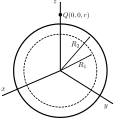
\includegraphics[width=0.5\linewidth]{figures/spherical-shell.pdf}
\caption{
    Spherical shell with inner and outer radii $R_1$ and $R_2$, respectively.
    The computation point $Q$ is located on the $z$ axis at a distance $r$ from
    the origin of the coordinates system.
    For our purposes we will assume that $Q$ is outside of the shell,
    i.e.\DIFaddbeginFL \DIFaddFL{~}\DIFaddendFL $r > R_2$.
}
\label{fig:spherical-shell}
\end{figure}

Consider a spherical shell with inner radius $R_1$ and outer radius $R_2$,
whose density is a function $\rho(r')$ of the radial coordinate
(Fig.\DIFaddbegin \DIFadd{~}\DIFaddend \ref{fig:spherical-shell}).
The gravitational potential generated by the shell on an arbitrary external
point $Q$ can be written as follows:

\begin{equation}
    V_\text{sh}(\phi, \lambda, r) = G
    \int\limits_0^{2\pi}
    \int\limits_{-\frac{\pi}{2}}^\frac{\pi}{2}
    \int\limits_{R_1}^{R_2}
    \frac{\rho(r')}{\ell} {r'}^2 \cos\phi' \,
    dr' d\phi' d\lambda',
\end{equation}

\noindent where $\ell$ is defined in equation\DIFaddbegin \DIFadd{~}\DIFaddend \ref{eq:ell}.

For $Q$ located along the $z$ axis (i.e., $\phi=90^\circ$) at a distance $r$ from the
origin, equation\DIFaddbegin \DIFadd{~}\DIFaddend \ref{eq:ell} simplifies to:

\begin{equation}
    \ell = \sqrt{r'^2 + r^2 - 2 r r' \sin\phi'}.
\end{equation}

\noindent
Because of the rotational symmetry along the $z$ \DIFdelbegin \DIFdel{axe}\DIFdelend \DIFaddbegin \DIFadd{axis}\DIFaddend , the integration in $\lambda'$ is
straightforward:

\begin{equation}
    V_\text{sh}(r) = 2\pi G
    \int\limits_{-\frac{\pi}{2}}^\frac{\pi}{2}
    \int\limits_{R_1}^{R_2}
    \frac{\rho(r') {r'}^2 \cos\phi'}{\sqrt{r'^2 + r^2 - 2 r r' \sin\phi'}}
    \, dr' d\phi',
\end{equation}

\noindent
while the integration in $\phi'$ can be performed independently of the density function.
Making use of SymPy \citep{sympy2017}, a Python library for symbolic mathematics, we
obtained the following expression for the potential:

\iftwocol{
\begin{equation}
    \begin{split}
        V_\text{sh}(r) = 2\pi G
        \int\limits_{R_1}^{R_2}
        \Big[ & \sqrt{r^2 + r'^2 + 2rr'} - \\
        & \sqrt{r^2 + r'^2 - 2rr'}
        \Big] \frac{r'\rho(r')}{r} \, dr'.
    \end{split}
\label{eq:shell-pot-sqrts}
\end{equation}
}{
\begin{equation}
    V_\text{sh}(r) = 2\pi G
    \int\limits_{R_1}^{R_2}
    \Big[ \sqrt{r^2 + r'^2 + 2rr'}  -
    \sqrt{r^2 + r'^2 - 2rr'}
    \Big] \frac{r'\rho(r')}{r} \, dr'.
\label{eq:shell-pot-sqrts}
\end{equation}
}

Because the computation point $Q$ is outside of the shell, $r > r'$ and the square roots
in equation\DIFaddbegin \DIFadd{~}\DIFaddend \ref{eq:shell-pot-sqrts} simplify to

\begin{equation}
    \sqrt{r^2 + r'^2 + 2rr'} = |r + r'| = r + r',
\end{equation}

\begin{equation}
    \sqrt{r^2 + r'^2 - 2rr'} = |r - r'| = r - r',
\end{equation}

\noindent which leads to the following expression for the potential:

\begin{equation}
    V_\text{sh}(r) = \frac{4\pi G}{r}
    \int\limits_{R_1}^{R_2} {r'}^2 \rho(r') \, dr'.
\label{eq:shell-pot}
\end{equation}

The gradient \DIFdelbegin \DIFdel{and the Marussi tensor }\DIFdelend of potentials that
depends solely on $r$ have only \DIFdelbegin \DIFdel{a few }\DIFdelend \DIFaddbegin \DIFadd{one }\DIFaddend non zero components: the vertical
component of the gradient ($g_z$)\DIFdelbegin \DIFdel{and the diagonal components of the
tensor ($g_{xx}$, $g_{yy}$, $g_{zz}$)}\DIFdelend .
Following \citet{Grombein2013}:

\begin{equation}
    g_z(r) = \frac{V_\text{sh}(r)}{r},
\DIFaddbegin \label{eq:shell-gz}
\DIFaddend \end{equation}

\DIFdelbegin \begin{displaymath}
    \DIFdel{g_{xx}(r) = g_{yy}(r) = -\frac{V_\text{sh}(r)}{r^2}
}\end{displaymath}%DIFAUXCMD
%DIFDELCMD < 

%DIFDELCMD < %%%
\begin{displaymath}
    \DIFdel{g_{zz}(r) = \frac{2V_\text{sh}(r)}{r^2}.
}\end{displaymath}%DIFAUXCMD
%DIFDELCMD < 

%DIFDELCMD < %%%
\DIFdelend From Eq.\DIFaddbegin \DIFadd{~}\DIFaddend \ref{eq:shell-pot} we can obtain expressions \DIFdelbegin \DIFdel{for }\DIFdelend \DIFaddbegin \DIFadd{of the }\DIFaddend gravitational potential for
different density functions.
\DIFaddbegin 

\subsection{\DIFadd{Linear density}}

\DIFaddend For a linear density function

\begin{equation}
    \rho(r') = ar' + b\ ,
\end{equation}

\noindent
the gravitational potential at any external point is

\begin{equation}
    V_\text{sh}^\text{lin}(r) = \pi G \left[
    a \frac{R_2^4 - R_1^4}{r} +
    b \,\frac{4}{3} \frac{R_2^3 - R_1^3}{r} \right].
    \label{eq:shell-pot-linear}
\end{equation}

\noindent The first term on this equation reproduces the potential generated
by a spherical shell with variable density $\rho(r') = ar'$, while the second
term constitutes the potential generated by a spherical shell with homogeneous
density $\rho = b$ \citep{Mikuska2006,Grombein2013}.
\DIFaddbegin \DIFadd{Eq~\ref{eq:shell-pot-linear} is in agreement with the one obtained by \mbox{%DIFAUXCMD
\citet{Lin2018}}\hspace{0pt}%DIFAUXCMD
.
}\DIFaddend 

\DIFdelbegin \DIFdel{An }\DIFdelend \DIFaddbegin \subsection{\DIFadd{Exponential density}}

\DIFadd{For an }\DIFaddend exponential density function
\DIFdelbegin \DIFdel{that assumes the values of $\rho_\text{out}$ and
$\rho_\text{in}$ on the shell's outer and inner surfaces, respectively, can be defined
as follows:
}\DIFdelend 

\begin{equation}
    \rho(r') = A e\DIFdelbegin \DIFdel{^{-(r' - R)/b} + C}\DIFdelend \DIFaddbegin \DIFadd{^{- k (r' - R)}}\DIFaddend ,
\end{equation}

\noindent
where \DIFaddbegin \DIFadd{$A$, $k$ and $R$ are constants, the gravitational potential on any external point
is
}\DIFaddend 

\begin{equation}
    \DIFdelbegin \DIFdel{A = (\rho_\text{in} - \rho_\text{out})
        }%DIFDELCMD < \left( %%%
\DIFdel{e^{( R_2 - R_1 )/b} - 1 }%DIFDELCMD < \right)%%%
\DIFdel{^{-1},
}\DIFdelend \DIFaddbegin \begin{split}
    V_\text{exp}(r) = \frac{4\pi G}{r} \frac{A}{k^3} \Big[
    & \left( R_1^2 k^2 + 2 R_1 k + 2 \right) e^{- k (R_1 - R)} - \\
    & \left( R_2^2 k^2 + 2 R_2 k + 2 \right) e^{- k (R_2 - R)}
    \Big].
    \end{split}
\DIFaddend \end{equation}


\DIFaddbegin \subsection{\DIFadd{Sinusoidal density}}

\DIFadd{For an sinusoidal density function
}

\DIFaddend \begin{equation}
    \DIFdelbegin \DIFdel{C = }\DIFdelend \rho\DIFdelbegin \DIFdel{_\text{out} - }\DIFdelend \DIFaddbegin \DIFadd{(r') = }\DIFaddend A \DIFaddbegin \DIFadd{\sin ( k (r' - R))}\DIFaddend ,
\end{equation}

\noindent
\DIFaddbegin \DIFadd{where $A$, $k$ and }\DIFaddend $R$ \DIFdelbegin \DIFdel{is the mean Earth radius, and $b$ is a constant
that determines the variability of the function: a low value of $b$
increases the maximum slope of the density function.
}%DIFDELCMD < 

%DIFDELCMD < %%%
\DIFdel{The analytical solution of the gravitational potential generated by a
spherical shell with a density function }\DIFdelend \DIFaddbegin \DIFadd{are constants, the gravitational potential on any external point
}\DIFaddend is

\begin{equation}
    \DIFdelbegin %DIFDELCMD < \begin{split}
%DIFDELCMD <         V_\text{sh}^\text{exp}(r) = \frac{4\pi G}{r}
%DIFDELCMD <         Ab
%DIFDELCMD <         \Big[
%DIFDELCMD <         & (R_1^2 + 2R_1 b + 2b^2)e^{-\frac{R_1 - R}{b}} - \\
%DIFDELCMD <         & (R_2^2 + 2R_2 b + 2b^2)e^{-\frac{R_2 - R}{b}}
%DIFDELCMD <         \Big] + \\
%DIFDELCMD <         & \frac{4 \pi G}{3 r} C (R_2^3 - R_1^3).
%DIFDELCMD <     \end{split}%%%
\DIFdelend \DIFaddbegin \begin{split}
    V_\text{sine}(r) = \frac{4\pi G}{r} \frac{A}{k^3} \Big[
    & (2 - k^2 R_2^2) \cos(k(R_2 - R)) + 2 k R_2 \sin(k(R_2 - R)) - \\
    & (2 - k^2 R_1^2) \cos(k(R_1 - R)) - 2 k R_1 \sin(k(R_1 - R))
        \Big]
    \end{split}\DIFaddend 
\DIFdelbegin %DIFDELCMD < \label{eq:shell-pot-exp}
%DIFDELCMD < %%%
\DIFdelend \end{equation}

\end{document}

